\documentclass[a4paper,12pt,oneside,openany]{book}	
\usepackage[utf8]{inputenc}
\usepackage[T1]{fontenc}
\usepackage{float}
\usepackage{listings}
\usepackage{xcolor}
\usepackage{tikz}
\usetikzlibrary{arrows.meta,positioning}
\usepackage[hidelinks]{hyperref}
\renewcommand{\figureautorefname}{Figura}
\renewcommand{\tableautorefname}{Tabela}
\renewcommand{\equationautorefname}{Equação}
\renewcommand{\appendixautorefname}{Apêndice}
\renewcommand{\chapterautorefname}{Capítulo}
\renewcommand{\sectionautorefname}{Seção}
\renewcommand{\subsectionautorefname}{Subseção}
\renewcommand{\subsubsectionautorefname}{Subseção}

% Setup for Python Code
\lstdefinestyle{pythonstyle}{
    language=Python,
    basicstyle=\ttfamily\small,
    keywordstyle=\color{blue},
    commentstyle=\color{gray},
    stringstyle=\color{orange},
    breaklines=true,
    frame=lines,
    captionpos=b
}

% Setup for Terminal/Text output
\lstdefinestyle{mystats}{
    basicstyle=\ttfamily\small,
    breaklines=true,
    frame=single,
    backgroundcolor=\color{lightgray!10}
}

\usepackage{layout}
\setlength{\textwidth}{15.0 cm}
\setlength{\textheight}{25.0 cm}


\usepackage[english,brazilian]{babel}
\usepackage{styles/pagina}	% pagina-padrao
\usepackage{styles/indentfirst}		% for indent
\usepackage{graphics,epsfig}
\usepackage{graphics}
\graphicspath{{./figuras/}}
\usepackage{pstricks,pst-node,pst-tree}
\usepackage{alltt}
%\usepackage{makeidx}
%\makeindex
\usepackage[figuresright]{styles/rotating} % for saydways tables and figures
\usepackage{enumerate}			% for configuration of enumerate environment
\usepackage{amsmath}
\usepackage{amssymb}
\usepackage{styles/portland}
\usepackage{multirow}

\setcounter{secnumdepth}{3}	% numeracao ate subsubsecao
\setcounter{tocdepth}{2}	% indice ate subsubsecao

\usepackage{longtable}


\begin{document}

\frontmatter
\thispagestyle{empty}

\input{frontmatter/Capa}

\pagebreak            

% Declaracao
\begin{center}
Declaração de Autoria e de Direitos
\end{center}

\vspace{0.5cm}

Eu, \emph{Hugo de Barros Araujo}, autor da monografia \emph{SISTEMAS MULTIAGENTE E APRENDIZADO POR REFORÇO APLICADOS A META-HEURÍSTICAS PARA OTIMIZAÇÃO DO PROBLEMA DE ROTEAMENTO DE VEÍCULOS COM JANELAS DE TEMPO}, subscrevo para os devidos fins, as seguintes informações:\\
1. O autor declara que o trabalho apresentado na disciplina de Projeto de Graduação da Escola Politécnica da UFRJ é de sua autoria, sendo original em forma e conteúdo.\\
2. Excetuam-se do item 1. eventuais transcrições de texto, figuras, tabelas, conceitos e idéias, que identifiquem claramente a fonte original, explicitando as autorizações obtidas dos respectivos proprietários, quando necessárias.\\
3. O autor permite que a UFRJ, por um prazo indeterminado, efetue em qualquer mídia de divulgação, a publicação do trabalho acadêmico em sua totalidade, ou em parte. Essa autorização não envolve ônus de qualquer natureza à UFRJ, ou aos seus representantes.\\
4. O autor pode, excepcionalmente, encaminhar à Comissão de Projeto de Graduação, a não divulgação do material, por um prazo máximo de 01 (um) ano, improrrogável, a contar da data de defesa, desde que o pedido seja justificado, e solicitado antecipadamente, por escrito, à Congregação da Escola Politécnica.\\
5. O autor declara, ainda, ter a capacidade jurídica para a prática do presente ato, assim como ter conhecimento do teor da presente Declaração, estando ciente das sanções e punições legais, no que tange a cópia parcial, ou total, de obra intelectual, o que se configura como violação do direito autoral previsto no Código Penal Brasileiro no art.184 e art.299, bem como na Lei 9.610.\\
6. O autor é o único responsável pelo conteúdo apresentado nos trabalhos acadêmicos publicados, não cabendo à UFRJ, aos seus representantes,  ou ao(s) orientador(es), qualquer responsabilização/ indenização nesse sentido.\\
7. Por ser verdade, firmo a presente declaração.\\

      \vspace{0.5cm}
      \begin{flushright}
         \parbox{10cm}{
            \hrulefill

            \vspace{-.375cm}
            \centering{Hugo de Barros Araujo}

            \vspace{0.1cm}
         }
      \end{flushright}
      
\pagebreak

% Copyright
      \vspace{0.5cm}

UNIVERSIDADE FEDERAL DO RIO DE JANEIRO \\
Escola Politécnica - Departamento de Eletrônica e de Computação \\
Centro de Tecnologia, bloco H, sala H-217, Cidade Universitária \\ 
Rio de Janeiro - RJ      CEP 21949-900\\
\vspace{0.5cm}
\paragraph{}Este exemplar é de propriedade da Universidade Federal do Rio de Janeiro, que poderá incluí-lo em base de dados, armazenar em computador, microfilmar ou adotar qualquer forma de arquivamento.
\paragraph{}É permitida a menção, reprodução parcial ou integral e a transmissão entre bibliotecas deste trabalho, sem modificação de seu texto, em qualquer meio que esteja ou venha a ser fixado, para pesquisa acadêmica, comentários e citações, desde que sem finalidade comercial e que seja feita a referência bibliográfica completa.
\paragraph{}Os conceitos expressos neste trabalho são de responsabilidade do(s) autor(es).


\pagebreak


% Agradecimento
\begin{center}
\textbf{AGRADECIMENTO}
\end{center}
      \vspace{0.5cm}

\paragraph{}Ao povo brasileiro, que financia esta universidade e tornou possível minha formação em uma instituição de excelência como a UFRJ. Que a educação pública, gratuita e de qualidade continue sendo um pilar de transformação, tornando-se cada vez mais inclusiva e acessível a todos.

\paragraph{}À minha família, a base de tudo o que sou. Um agradecimento profundo e especial aos meus pais, José Antonio e Rosália, que não mediram esforços para que eu chegasse até aqui. O apoio incondicional, os sacrifícios silenciosos e o incentivo constante foram o combustível necessário para concluir esta jornada. Vocês são meu maior exemplo de dedicação e amor.

\paragraph{}Ao meu tio e padrinho, Lorran, quem mais me ajudou a despertar o gosto pela ciência.

\paragraph{}À minha namorada, Eduarda, parceira de todas as horas. Obrigado por compartilhar a vida comigo, por deixar tudo sempre leve e alegre quando estou com você.


\pagebreak


% Resumo
\begin{center}
\textbf{RESUMO}
\end{center}
      \vspace{0.5cm}

\paragraph{}Este trabalho aborda a resolução do Problema de Roteamento de Veículos com Janelas de Tempo (\textit{Vehicle Routing Problem with Time Windows} - VRPTW), um desafio de otimização combinatória classificado como \textit{NP-hard}, cujas aplicações práticas são fundamentais para a eficiência logística e redução de custos operacionais. O objetivo central é o desenvolvimento de um sistema híbrido que integra meta-heurísticas clássicas a um Sistema Multiagente (\textit{Multi-Agent System} - MAS) orquestrado por Aprendizado por Reforço (\textit{Reinforcement Learning} - RL). Inicialmente, foram implementados de forma independente os algoritmos de \textit{Simulated Annealing}, \textit{Tabu Search}, e \textit{Genetic Algorithm}, utilizando as instâncias de Solomon como \textit{benchmark} para avaliação de desempenho.

\paragraph{}A originalidade da proposta reside na encapsulação desses algoritmos como agentes especialistas dentro do \textit{framework} Mesa, onde a cooperação é estabelecida através de uma base de soluções de elite e da estratégia de \textit{Path Relinking}, que explora trajetórias entre soluções de alta qualidade para evitar ótimos locais. Para elevar a eficiência do sistema, aplicou-se o algoritmo \textit{Q-Learning} como uma hiper-heurística capaz de aprender, de forma autônoma, qual especialista deve ser acionado em diferentes estados do espaço de busca. Os resultados sugerem que a inteligência coletiva e a adaptação dinâmica de parâmetros via RL superam o desempenho individual dos algoritmos, proporcionando soluções otimizadas em tempo computacional viável.

\begin{description}
    \item[Palavras-chave:]  Otimização Combinatória, VRPTW, Sistemas Multiagentes, Meta-heurísticas, Aprendizado por Reforço, \textit{Path Relinking}.
\end{description}

\pagebreak


% Abstract
\begin{center}
\textbf{ABSTRACT}
\end{center}
      \vspace{0.5cm}

\paragraph{}This work addresses the resolution of the Vehicle Routing Problem with Time Windows (VRPTW), a NP-hard combinatorial optimization challenge with critical applications in logistics efficiency and operational cost reduction. The primary objective is to develop a hybrid system that integrates classical metaheuristics within a Multi-Agent System (MAS) orchestrated by Reinforcement Learning (RL). Initially, Simulated Annealing, Tabu Search, and Genetic Algorithms were independently implemented and evaluated using Solomon’s benchmark instances to establish performance baselines.

\paragraph{}The originality of this approach lies in encapsulating these algorithms as specialized agents within the Mesa framework, where cooperation is established through a shared elite solution pool and the Path Relinking strategy, which explores trajectories between high-quality solutions to circumvent local optima. To enhance system efficiency, the Q-Learning algorithm was applied as a hyper-heuristic capable of autonomously learning which specialist to activate across different states of the search space. Preliminary results suggest that collective intelligence and dynamic parameter adaptation via RL outperform individual algorithmic performance, providing optimized solutions within viable computational time.


\begin{description}
    \item[Key-words:] Combinatorial Optimization, VRPTW, Multi-Agent Systems, Metaheuristics, Reinforcement Learning, Path Relinking.
\end{description}


\pagebreak


% Siglas
\begin{center}
\textbf{SIGLAS}
\end{center}
      \vspace{0.5cm}

\paragraph{}GA -- \textit{Genetic Algorithm} (algoritmo genético)
\paragraph{}I/O -- \textit{In/Out} (entrada/saída)
\paragraph{}MAS -- \textit{Multi-Agent System} (sistema multi-agente)
\paragraph{}MAS-RL -- \textit{Multi-Agent System with Reinforcement Learning} (sistema multi-agente com aprendizado por reforço)
\paragraph{}NP-hard -- \textit{Non-deterministic Polynomial-time hard} (problemas de tempo polinomial não-determinístico difícil)
\paragraph{}OOP -- \textit{Object-Oriented Programming} (programação orientada a objetos)
\paragraph{}PR -- \textit{Path Relinking} (reconexão por caminhos)
\paragraph{}RAM -- \textit{Random Access Memory} (memória de acesso aleatório)
\paragraph{}RL -- \textit{Reinforcement Learning} (aprendizado por reforço)
\paragraph{}SA -- \textit{Simulated Annealing} (recozimento simulado)
\paragraph{}TS -- \textit{Tabu Search} (busca tabu)
\paragraph{}TSP -- \textit{Traveling Salesman Problem} (problema do caixeiro viajante)
\paragraph{}UFRJ -- Universidade Federal do Rio de Janeiro
\paragraph{}VRP -- \textit{Vehicle Routing Problem} (problema de roteamento de veículos)
\paragraph{}VRPTW -- \textit{Vehicle Routing Problem with Time Windows} (problema de roteamento de veículos com janelas de tempo)

\pagebreak









% Table of Contents
% ---------------------------------------------------------------
     \tableofcontents
% ---------------------------------------------------------------
% Lista de figuras
% ---------------------------------------------------------------
%\cleardoublepage
%\addcontentsline{toc}{chapter}{Lista de Figuras}
\listoffigures
% ---------------------------------------------------------------
% Lista de Tabelas
% ---------------------------------------------------------------
%\cleardoublepage
%\addcontentsline{toc}{chapter}{Lista de Tabelas}
\listoftables

\mainmatter
\cleardoublepage
% ---------------------------------------------------------------
% Chapter 1 - Introdução
% ---------------------------------------------------------------
\chapter{Introdução}
\label{cap1}
\paragraph{}Este capítulo introduz o leitor ao contexto no qual a presente pesquisa se insere, apresentando as motivações iniciais, o escopo do problema de otimização selecionado e a relevância científica da abordagem proposta. A \autoref{sec:tema} delineia o tema central do estudo, abordando as restrições e a hierarquia do Problema de Roteamento de Veículos com Janelas de Tempo (VRPTW). Em seguida, a \autoref{sec:delimitacao} estabelece as delimitações do trabalho, focando no desenvolvimento e avaliação empírica de meta-heurísticas integradas em um sistema multi-agente colaborativo guiado por aprendizado por reforço. A justificativa para a aplicação destas ferramentas algorítmicas, dadas as dificuldades inerentes aos métodos exatos diante de problemas classificados como \textit{NP-hard}, é apresentada na \autoref{sec:justificativa}. Por fim, as Seções \ref{sec:objetivos}, \ref{sec:metodologia} e \ref{sec:descricao} expõem, respectivamente, os objetivos formulados, a metodologia adotada de melhoria contínua e a estruturação capitular do conteúdo subsequente neste documento.

\section{Tema}
\label{sec:tema}

\paragraph{}O tema do trabalho é a aplicação e a análise de métodos meta-heurísticos para a resolução de problemas de otimização complexos, classificados como \textit{NP-hard} \cite{Garey79}, como o Problema de Roteamento de Veículos (ou \textit{Vehicle Routing Problem} -- VRP). O VRP, introduzido pioneiramente na literatura sob a ótica da distribuição de derivados de petróleo em 1959 \cite{Dantzig59}, consiste em determinar o conjunto ideal de rotas para uma frota de veículos, com o objetivo de visitar um conjunto de clientes, cada um com uma demanda específica. O problema a ser resolvido é encontrar a solução mais eficiente para este roteamento, considerando restrições como distância total, número de veículos, tempo e capacidade de entrega.

\paragraph{}Dentro do vasto domínio do VRP, este trabalho concentra-se especificamente no Problema de Roteamento de Veículos com Janelas de Tempo (\textit{Vehicle Routing Problem with Time Windows} -- VRPTW). O VRPTW estende o problema clássico ao impor que o atendimento a cada cliente deve ser iniciado obrigatoriamente dentro de um intervalo temporal pré-definido, composto por um tempo de abertura e um tempo de fechamento (\textit{time window}).



\paragraph{}A inclusão destas restrições temporais torna o desafio ainda mais rigoroso, pois a viabilidade de uma rota não depende apenas da capacidade de carga do veículo, mas da coordenação precisa dos horários de chegada e dos tempos de serviço em cada nó. Neste cenário, o objetivo de encontrar a solução mais eficiente desdobra-se em uma hierarquia de otimização: busca-se, primordialmente, a minimização do número de veículos necessários e, subsequentemente, a redução da distância total percorrida, garantindo que nenhum compromisso temporal seja violado. Por ser um problema de natureza \textit{NP-hard}, a exploração de janelas de tempo exige que os métodos meta-heurísticos aplicados possuam alta capacidade de adaptação para navegar em um espaço de busca repleto de restrições de inviabilidade.

\section{Delimitação}
\label{sec:delimitacao}

\paragraph{}O objeto de estudo são problemas de otimização \textit{NP-hard}. O projeto se concentrará na otimização do VRPTW, que estende o clássico Problema do Caixeiro Viajante (\textit{Traveling Salesman Problem} -- TSP) para múltiplos veículos, capacidade de carga e janelas de tempo. O foco será na implementação e comparação de diferentes algoritmos meta-heurísticos (\textit{Simulated Annealing} -- SA, \textit{Tabu Search} -- TS e \textit{Genetic Algorithm} -- GA), e na integração desses métodos com um sistema multiagente (\textit{Multi-Agent System} -- MAS), conjuntamente com a aplicação de aprendizado por reforço (\textit{Reinforcement Learning} -- RL) para melhoria deste sistema.

\section{Justificativa}
\label{sec:justificativa}

\paragraph{}O VRPTW, em virtude de sua formulação que estende o VRP clássico, é rigorosamente classificado como um problema \textit{NP-hard} \cite{Garey79}. Nesse contexto de alta complexidade computacional, o esforço temporal demandado por métodos exatos para a obtenção de uma solução ótima cresce de forma exponencial em função da dimensionalidade da instância analisada, tornando tais abordagens intratáveis para a ampla escala de cenários reais. Diante dessa limitação, as meta-heurísticas despontam como uma alternativa viável, visto que, embora não assegurem a otimalidade global, oferecem mecanismos para explorar o espaço de busca eficientemente, fornecendo aproximações de alta qualidade em tempo computacional factível.

\paragraph{}A originalidade deste trabalho reside na aplicação de um MAS com RL para integrar e aprimorar o desempenho dos diferentes métodos meta-heurísticos. O objetivo é explorar como a comunicação entre agentes pode levar a resultados superiores aos de cada algoritmo individualmente, evitando mínimos locais e alcançando uma solução globalmente mais eficiente. A importância do projeto está em sua aplicabilidade prática em áreas como logística, transporte e serviços de entrega, onde a otimização de rotas é fundamental para a eficiência e redução de custos.

\paragraph{}Ainda no tocante à justificativa da abordagem, o Apêndice B apresenta uma análise quantitativa da grandeza temporal requerida pela força bruta para a obtenção da solução ótima nas instâncias discutidas, reiterando a necessidade de métodos heurísticos.

\section{Objetivos}
\label{sec:objetivos}

\paragraph{}O objetivo geral é analisar e implementar um sistema híbrido, combinando métodos meta-heurísticos com um sistema multiagente e aprendizado por reforço, para otimizar a resolução do VRPTW. Como objetivos específicos, temos:

\begin{enumerate}
    \item Formular o VRPTW, definindo a função de custo e as restrições (tempo, volume, peso) para a avaliação das soluções;
    \item Implementar, de forma independente, os algoritmos meta-heurísticos: SA, TS e GA;
    \item Integrar os algoritmos em um MAS, no qual a interação entre os agentes leva à colaboração na busca pela solução;
    \item Aplicar RL para aprimorar a estratégia de busca dos agentes;
    \item Comparar o desempenho dos algoritmos individuais com o MAS e o sistema com aprendizado por reforço (MAS-RL) para avaliar a melhoria na otimização da solução.
\end{enumerate}

\section{Metodologia}
\label{sec:metodologia}

\paragraph{}A metodologia será dividida nas seguintes etapas, focando na aplicação de uma abordagem iterativa e de melhoria contínua para a otimização do problema.

\begin{itemize}
    \item \textbf{Modelagem do Problema:} O VRP será formulado como um problema de otimização, no qual uma solução é representada como um vetor ordenado de pontos de entrega. A função de custo avaliará a qualidade de cada solução, considerando a distância percorrida, o número de veículos e as restrições de tempo e capacidade, atribuindo pesos a cada parâmetro;
    \item \textbf{Implementação dos Algoritmos:} Os três algoritmos meta-heurísticos serão implementados em \textit{Python}. Para cada algoritmo, serão definidas etapas de inicialização de uma solução aleatória, geração de novas soluções e a manutenção de um histórico para direcionar a busca;
    \item \textbf{Integração com Sistema Multiagente:} Os algoritmos serão encapsulados como agentes dentro de um MAS. O sistema operará de forma cooperativa, permitindo que os agentes interajam para compartilhar informações e refinar as soluções encontradas;
    \item \textbf{Aplicação de Aprendizado por Reforço:} O método de \textit{Q-Learning} será aplicado para associar os estados do problema às ações (ajuste de estratégias de busca), permitindo que o sistema aprenda a selecionar a melhor abordagem de forma autônoma ao longo do tempo.
\end{itemize}



\section{Descrição}
\label{sec:descricao}

\paragraph{}O restante deste trabalho está organizado em quatro capítulos principais, além das referências bibliográficas e apêndices, conforme detalhado a seguir.

\paragraph{}No Capítulo 2, é apresentada a Fundamentação Teórica, que estabelece a base conceitual necessária para a compreensão do projeto. Nele, define-se o VRPTW e detalha-se a metodologia de avaliação baseada no \textit{Benchmark} de Solomon \cite{Solomon87}. O capítulo descreve o funcionamento técnico do trio de meta-heurísticas selecionado e introduz a arquitetura do MAS utilizando o \textit{framework} Mesa. Finaliza abordando as estratégias de cooperação via \textit{Path Relinking} (PR) e a teoria de Aprendizado por Reforço.

\paragraph{}O Capítulo 3 detalha o desenvolvimento do Método Proposto da pesquisa. Ele descreve as etapas iniciais de modelagem e as arquiteturas das classes. Em seguida, expõe-se a modelagem do sistema multiagente, demonstrando a dinâmica de cooperação por meio do \textit{Path Relinking} e a implementação do \textit{Q-Learning} como hiper-heurística, orquestrando e selecionando as melhores ações para esse ambiente.

\paragraph{}Os testes realizados e a apresentação dos resultados ficam a encargo do Capítulo 4: Experimentos Computacionais. A seção avalia o desempenho prático, apresentando inicialmente o \textit{baseline} de cada meta-heurística isolada, em sequência os resultados agregados pela cooperação simplista do sistema multiagente e, por fim, a análise do desempenho da hiper-heurística com Aprendizado por Reforço (MAS-RL).

\paragraph{}As reflexões e fechamentos a respeito da pesquisa são apresentados no Capítulo 5, que compõe as Conclusões do trabalho. Nele, será explicitado se a integração entre MAS e RL de fato superou o desempenho dos algoritmos isolados, validando a hipótese de que a inteligência coletiva e a adaptação dinâmica de parâmetros produzam soluções superiores para o VRPTW. O capítulo encerra com a indicação de oportunidades de melhoria e sugestões para trabalhos futuros.

% ---------------------------------------------------------------
% Chapter 2 - Fundamentação Teórica
% ---------------------------------------------------------------
\chapter{Fundamentação Teórica}
\label{cap2}
\paragraph{}Este capítulo apresenta a fundamentação teórica essencial para o entendimento das metodologias e soluções computacionais propostas neste trabalho. A \autoref{sec:def_problema} apresenta o conceito do Problema de Roteamento de Veículos, detalha os padrões de avaliação de instâncias da literatura e formaliza-o matematicamente. A \autoref{sec:selecao_meta} apresenta as meta-heurísticas adotadas (Recozimento Simulado, Busca Tabu e Algoritmo Genético) descrevendo sucintamente seus funcionamentos e premissas. Posteriormente, a \autoref{sec:sma} explora os princípios de um Sistema multiagente, abordando o \textit{framework} de modelagem distribuída escolhido e a estratégia de cooperação implementada, o \textit{Path Relinking}. A compreensão do Aprendizado por Reforço e a lógica da recompensa empregada na estratégia do \textit{Q-Learning}, que norteia a coordenação estratégica proposta, são objetos da \autoref{sec:rl}. Por fim, a \autoref{sec:avaliacao_estatistica} discute a importância de uma avaliação estatística rigorosa para a comparação de algoritmos meta-heurísticos, destacando os testes de hipóteses adequados para validar as conclusões obtidas a partir dos experimentos computacionais realizados.

\section{Definição do problema}
\label{sec:def_problema}

\paragraph{}Para compreender a avaliação das soluções quantitativas na experimentação futura, faz-se necessário contextualizar a natureza exata e as particularidades do problema central que pauta toda a sequência teórica e empírica deste estudo. Inicialmente, a \autoref{sec:vrp} define o arranjo lógico do conhecido e amplamente mapeado VRP, englobando as dificuldades computacionais e as raízes atadas à complexidade tempo de polinomial não-determinístico difícil (\textit{NP-hard}). Secundariamente, a \autoref{sec:benchmark} elucida a base paramétrica de referências extraída do Benchmark de Solomon de 1987, estabelecendo um padrão ouro viável de contraste na apuração da acurácia e otimização obtida pelas composições desenvolvidas em tempo de execução comparado.

\subsection{O Problema de Roteamento de Veículos}
\label{sec:vrp}

\paragraph{} O Problema de Roteamento de Veículos (VRP) é um desafio de otimização combinatória e programação linear inteira que busca determinar o conjunto ideal de rotas para uma frota de veículos entregarem mercadorias a um conjunto específico de clientes \cite{Dantzig59, Vidal20}. De forma genérica, o objetivo fundamental do VRP é minimizar o custo total da operação (geralmente expresso em distância total ou tempo) garantindo que:

\begin{itemize}
    \item Cada cliente deve ser visitado exatamente uma vez;
    \item Todos os veículos devem começar e terminar suas rotas em um depósito central;
    \item As restrições operacionais (como capacidade de carga ou janelas de tempo) devem ser estritamente respeitadas.
\end{itemize}

\paragraph{} O VRP é classificado na teoria da complexidade computacional como um problema \textit{NP-hard} (\textit{Non-deterministic Polynomial-time hard}) \cite{Garey79}. Do ponto de vista teórico, isso implica que qualquer problema pertencente à classe de complexidade \textit{NP} (\textit{Non-deterministic Polynomial}) pode ser reduzido ao VRP por meio de uma transformação em tempo polinomial. Na prática, isso significa que, a menos que $P = NP$, não se conhece nenhum algoritmo determinístico capaz de encontrar a solução ótima para o problema em tempo polinomial. É precisamente essa complexidade computacional inerente que fundamenta a aplicação das meta-heurísticas (SA, TS e GA) investigadas neste estudo. Em contraste com os métodos de resolução exatos, as abordagens meta-heurísticas são concebidas para encontrar soluções subótimas de alta qualidade em um tempo de processamento que viabilize a aplicação prática em cenários de envergadura real.

\subsection{Metodologia de avaliação e o Benchmark de Solomon}
\label{sec:benchmark}

\paragraph{}Para assegurar a validade científica deste estudo e permitir a comparabilidade dos resultados obtidos pelas meta-heurísticas propostas, a modelagem será conduzida estritamente sob os parâmetros do Benchmark de Solomon (1987). A utilização de instâncias consagradas na literatura é imperativa, pois fornecem um ``gabarito'' técnico que permite atestar a precisão e a eficiência de cada algoritmo desenvolvido.

\paragraph{}Dado que as instâncias de Solomon incorporam coordenadas geográficas, demandas de carga e janelas temporais, o problema aqui tratado é classificado como Problema de Roteamento de Veículos com Janelas de Tempo (VRPTW). Embora simplificada em relação às complexidades imprevisíveis do mundo real (como variações de tráfego ou clima), essa modelagem oferece um ambiente controlado e puramente matemático para a análise de desempenho algorítmico. Para que a comparação seja viável e metodologicamente aceitável, o instanciação seguirá as métricas rigorosas do \textit{benchmark}:

\begin{enumerate}
    \item \textbf{Função Objetivo Hierárquica:} A avaliação do desempenho seguirá uma prioridade de dois níveis:
    \begin{enumerate}
        \item \textbf{Minimização do número de veículos ($K$):} O objetivo primário é atender a todos os clientes com a menor frota possível.
        \item \textbf{Minimização da distância total percorrida ($D$):} Como objetivo secundário, busca-se o percurso mais curto para a frota definida.
    \end{enumerate}

    \item \textbf{Cálculo de Distância e Tempo:} A distância entre dois pontos $(i, j)$ é calculada pela Distância Euclidiana plana:
    
    $$d_{ij} = \sqrt{(x_i - x_j)^2 + (y_i - y_j)^2}$$

    \item Conforme as regras de Solomon, o tempo de viagem é numericamente equivalente à distância ($t_{ij} = d_{ij}$), e todos os cálculos devem utilizar precisão dupla (\textit{double precision}), com os resultados finais de distância arredondados para duas casas decimais.

    \item \textbf{Ponto de Origem e Retorno:} O cliente indexado como 0 define o depósito central, ponto obrigatório de partida e encerramento de todas as rotas.
    
    \item \textbf{Restrições de Viabilidade:} Uma solução para o problema é considerada válida apenas se garantir o atendimento da demanda de todos os clientes em sua totalidade. Além disso, cada rota individual deve respeitar rigorosamente as seguintes restrições operacionais: a soma das demandas dos clientes inseridos em uma mesma rota não pode exceder a Capacidade Máxima do Veículo ($Q$); e o serviço deve ser iniciado e finalizado dentro da Janela de Tempo estabelecida pelo cliente (\textit{Ready Time} e \textit{Due Date}), computando-se obrigatoriamente o Tempo de Serviço (\textit{Service Time}) em cada parada.
\end{enumerate}

\paragraph{}Esta abordagem padronizada transforma o problema em um estudo de caráter matemático e exploratório, estabelecendo uma base sólida que pode, futuramente, ser adaptada para modelos logísticos de maior complexidade e variáveis dinâmicas.

\subsection{Formulação Matemática}
\label{sec:modelo_milp}

\paragraph{} Para formalizar o VRPTW e estabelecer o modelo de referência deste trabalho, apresenta-se a seguir uma formulação de Programação Linear Inteira Mista (MILP -- \textit{Mixed-Integer Linear Programming}).

\paragraph{} Considere um grafo direcionado $G = (V, A)$, onde $V = \{0, 1, \dots, n, n+1\}$ é o conjunto de vértices e $A$ representa o conjunto de arcos válidos, livre de laços conexos ao próprio nó (\textit{self-loops}). Os vértices $0$ e $n+1$ delimitam geometricamente o depósito central em suas instâncias de partida e chegada, respectivamente, enquanto o subconjunto $C = \{1, \dots, n\}$ define os nós de demanda associados aos clientes. Para cada cliente $i \in C$, estipula-se uma demanda de carga $q_i$, um tempo de serviço fixo $s_i$ e uma janela temporal de atendimento restrita ao intervalo $[e_i, l_i]$. Cada arco $(i, j) \in A$ carrega um custo de percurso $c_{ij}$ e um tempo de deslocamento $t_{ij}$. 

\paragraph{} Para garantir que o tamanho da frota disponível $|K|$ atue estritamente como uma cota superior e não como uma imposição de despacho mandatória, o conjunto de arcos $A$ inclui explicitamente o arco direcionado virtual $(0, n+1)$, cujos parâmetros são zerados ($c_{0, n+1} = 0$ e $t_{0, n+1} = 0$). Desse modo, qualquer veículo homogêneo $k \in K$ que permaneça ocioso cumpre os requisitos de partida e chegada realizando a trajetória direta entre os depósitos virtuais sem penalizar a função objetivo. 

\paragraph{} O modelo adota duas classes de variáveis de decisão: a variável binária $x_{ijk}$, que assume valor 1 se o veículo $k \in K$ percorre diretamente o arco $(i, j) \in A$, e 0 caso contrário; e a variável contínua $w_i \ge 0$, que estipula o instante de início do serviço no vértice $i \in V$. A formulação matemática exata é estruturada conforme segue:

\begin{align}
\text{Minimizar} \quad & Z = \sum_{k \in K} \sum_{(i,j) \in A} c_{ij}\, x_{ijk}
  \label{eq:obj}\\[4pt]
\text{Sujeito a:} \quad
& \sum_{k \in K} \sum_{j:(i,j)\in A} x_{ijk} = 1,
  && \forall i \in C \label{eq:grau}\\[2pt]
& \sum_{j:(0,j)\in A} x_{0jk} = 1,
  && \forall k \in K \label{eq:saida}\\[2pt]
& \sum_{i:(i,h)\in A} x_{ihk} - \sum_{j:(h,j)\in A} x_{hjk} = 0,
  && \forall h \in C,\ \forall k \in K \label{eq:fluxo}\\[2pt]
& \sum_{i:(i,n+1)\in A} x_{i,n+1,k} = 1,
  && \forall k \in K \label{eq:chegada}\\[2pt]
& \sum_{i \in C} q_i \sum_{j:(i,j)\in A} x_{ijk} \le Q,
  && \forall k \in K \label{eq:cap}\\[2pt]
& w_i + s_i + t_{ij} - M_{ij}\bigl(1 - \textstyle\sum_{k\in K} x_{ijk}\bigr) \le w_j,
  && \forall (i,j) \in A \label{eq:tempo}\\[2pt]
& e_i \le w_i \le l_i,
  && \forall i \in V \label{eq:janela}\\[2pt]
& x_{ijk} \in \{0,1\},
  && \forall (i,j) \in A,\ \forall k \in K \label{eq:dominio}
\end{align}

\paragraph{} A função objetivo \eqref{eq:obj} visa minimizar o custo total de deslocamento da frota. A restrição de grau \eqref{eq:grau} impõe que cada nó de cliente seja visitado exatamente uma vez por um único veículo. As restrições \eqref{eq:saida}, \eqref{eq:fluxo} e \eqref{eq:chegada} gerenciam as leis de conservação de fluxo, obrigando que todo veículo ativado saia do depósito inicial $0$, preserve a continuidade física ao transitar por nós intermediários de clientes e finalize seu percurso no depósito de encerramento $n+1$. 

\paragraph{} Os limites físicos de carregamento de cada veículo são controlados pela inequação \eqref{eq:cap}. A coordenação cronológica e a eliminação de subrotas disjuntas (\textit{subtour elimination}) são coordenadas pelas expressões \eqref{eq:tempo} e \eqref{eq:janela}. A fim de prover um relaxamento linear computacionalmente mais restritivo e robusto se comparado ao uso de uma constante global arbitrária, a Equação \eqref{eq:tempo} adota um coeficiente penalizador Big-$M$ indexado localmente, parametrizado por $M_{ij} = \max\{0, l_i + s_i + t_{ij} - e_j\}$. Por fim, a restrição \eqref{eq:janela} delimita as fronteiras operacionais das janelas de tempo de cada vértice.

\paragraph{Relação com a Abordagem Heurística}

\paragraph{} Determinar a solução ótima do modelo MILP por meio de métodos exatos é uma tarefa intratável para problemas de grande porte devido à classificação do VRPTW como um problema \textit{NP-Hard}. Frente a essa limitação, este trabalho recorre a abordagens meta-heurísticas para guiar a busca por soluções de alta qualidade.

\paragraph{} Sob a perspectiva algorítmica, o espaço de busca e a validação das restrições matemáticas sofrem uma reconfiguração metodológica, dividindo-se em dois pilares:
\begin{enumerate}
    \item \textbf{Atendidas por construção via representação:} Ao contrário dos solucionadores exatos, que avaliam tensores de adjacência infactíveis durante o processo de ramificação, os algoritmos heurísticos propostos eliminam a necessidade de lidar com inviabilidades de rota. As restrições de conservação de fluxo \eqref{eq:saida}-\eqref{eq:chegada}, capacidade \eqref{eq:cap}, sincronismo temporal \eqref{eq:tempo} e janelas de atendimento \eqref{eq:janela} são asseguradas de forma intrínseca pela estrutura de codificação adotada, impossibilitando o software de gerar um plano de transporte operacionalmente inválido.
    \item \textbf{Aproximadas empiricamente:} A otimização estrita da função objetivo \eqref{eq:obj} deixa de ser avaliada sob uma perspectiva global fechada. O custo total e o dimensionamento da frota passam a ser minimizados de forma empírica por meio da dinâmica cooperativa e competitiva dos operadores estocásticos, os quais sacrificam a prova matemática de otimalidade em prol da viabilidade de tempo de execução computacional.
\end{enumerate}


\subsection{Representação de soluções: O paradigma de \textit{giant tour}}
\label{subsec:giant_tour}

\paragraph{} O fator determinante para o desempenho de meta-heurísticas aplicadas ao VRPTW reside na escolha da estrutura de dados empregada para codificar uma solução. A manipulação direta da álgebra linear exata apresentada na \autoref{sec:modelo_milp} por operadores estocásticos impõe barreiras geométricas intransponíveis à convergência dos algoritmos. Para contornar essa restrição estrutural, a literatura de Pesquisa Operacional frequentemente adota o paradigma de representação baseado em rotas gigantes, ou \textit{giant tours}.

\paragraph{} Proposto por \cite{prins2004simple}, o conceito de \textit{giant tour} consiste em transpor uma solução complexa multirrota do VRP para uma única sequência linear e contínua contendo a totalidade dos $n$ clientes mapeados, omitindo as inserções intermediárias do depósito central. Essa abstração permite que o problema de roteamento seja operado temporariamente sob as propriedades de uma permutação pura do Problema do Caixeiro Viajante. Consequentemente, as meta-heurísticas concentram seus mecanismos de busca exclusivamente na identificação da sequência de atendimento global ideal, explorando um espaço amostral significativamente mais denso e homogêneo.

\paragraph{} A restauração da viabilidade logística e a conversão do arranjo unidimensional em um plano de expedição multifrota ocorrem por meio de um decodificador de partição, denominado fatiamento ou \textit{split}. Neste projeto, codificou-se uma variante estabelecida sob o princípio da divisão gulosa (\textit{greedy split}), cuja execução ocorre de forma sequencial adjacente ao \textit{giant tour}. O algoritmo realiza a varredura progressiva da lista, acumulando as demandas de carga e os tempos de chegada nos nós. No instante exato em que a transição para o cliente subsequente acusa a iminência de violação dos limites de capacidade do veículo \eqref{eq:cap} ou estouramento do limite superior da janela temporal \eqref{eq:janela}, o decodificador força dinamicamente o retorno do veículo atual ao depósito central e despacha uma nova unidade para dar continuidade ao atendimento.

\paragraph{} Posto que o retorno ao depósito é desencadeado de forma reativa e automática diante de uma saturação operacional, evidencia-se que a totalidade das rotas fatiadas é viável por construção, eliminando por completo a ocorrência de soluções logísticas inválidas ao longo dos passos do algoritmo. No entanto, essa simplificação estrutural introduz um compromisso metodológico (\textit{trade-off}) que deve ser formalizado como uma limitação assumida do modelo. Devido ao caráter míope inerente à partição gulosa, que efetua os cortes de rota de maneira imediata sem mensurar o impacto combinatório dessa quebra nas demandas remanescentes, o procedimento tende a superestimar o número total de veículos ($K$) necessários para consolidar a frota final. Trata-se de uma fragilidade conhecida, tolerada institucionalmente em favor da robustez estrutural e da velocidade de convergência computacional das meta-heurísticas em problemas de larga escala.

\section{Meta-heurísticas selecionadas}
\label{sec:selecao_meta}

\paragraph{}As meta-heurísticas Recozimento Simulado, Busca Tabu e Algoritmo Genético são clássicas no contexto do VRP, portanto adequadas para o presente estudo. A diversidade técnica entre esses métodos permite utilizar diferentes mecanismos de escape de ótimos locais e estratégias de exploração do espaço de busca diante das restrições de roteamento. A seguir, serão apresentados os fundamentos do funcionamento de cada um deles.

\subsection{Recozimento Simulado}
\label{sec:sa}

\paragraph{} Explora possíveis soluções por meio de um mecanismo probabilístico inspirado no processo de resfriamento de metais \cite{Kirkpatrick83}. Se $\Delta f$ é a diferença de custo entre a nova solução ($s'$) e a atual ($s$):

$$\Delta f = f(s') - f(s)$$

\vspace{0.5cm}
\noindent a probabilidade $P$ de aceitação é definida por:

$$P(\text{aceitar } s') = 
\begin{cases} 
1, & \text{se } \Delta f < 0 \\
e^{-\frac{\Delta f}{T}}, & \text{se } \Delta f \geq 0 
\end{cases}$$

\vspace{0.5cm}
\noindent onde $T$ é a temperatura, que decai ao longo do tempo conforme uma taxa de resfriamento $\alpha$:

$$T_{k+1} = \alpha \cdot T_k$$

\subsection{Busca Tabu}
\label{sec:ts}

\paragraph{} O método utiliza ``listas tabu'', que impedem o algoritmo de retornar a soluções visitadas recentemente, forçando uma exploração sistemática e agressiva de novas vizinhanças \cite{Glover89}. Mais objetivamente, o algoritmo opera sobre a vizinhança $N(s)$ da solução atual, mas subtrai os movimentos que estão na Lista Tabu ($L$):

$$s_{next} = \text{argmin} \{f(s') \mid s' \in N(s) \setminus L\}$$

\paragraph{}Entretanto, existe o Critério de Aspiração. Se uma solução $s'$ está na lista tabu, mas seu custo é melhor que a melhor solução encontrada até agora ($s_{best}$), o estado tabu é ignorado:

$$\text{Se } f(s') < f(s_{best}), \text{ então } s' \in \textit{Candidatos} \text{ mesmo se } s' \in L$$

\subsection{Algoritmo Genético}
\label{sec:ga}

\paragraph{} Por meio dos operadores de cruzamento, mutação e seleção, o algoritmo é capaz de recombinar sub-rotas eficientes de diferentes soluções para gerar descendentes potencialmente superiores \cite{Holland75, Goldberg89}. Isso se traduz em converter o problema de minimização de custos em um valor de sobrevivência, representado pela função de aptidão (\textit{fitness}) $F(s)$:

$$F(s) = \frac{1}{C(s) + \epsilon}$$

\vspace{0.5cm}
\noindent onde $\epsilon$ é um valor infinitesimal para evitar divisão por zero. Presente, neste caso, apenas por rigor teórico, pois a função de custo que será utilizada é sempre maior que 0. A probabilidade de um indivíduo ser selecionado para o cruzamento é dada por:

$$P_i = \frac{F(s_i)}{\sum_{j=1}^{N} F(s_j)}$$

\vspace{0.5cm}
\noindent onde $N$ é o tamanho da população. Isso garante que rotas mais curtas tenham maior probabilidade biológica de transmitir seus genes (sequências de clientes).


\section{Sistema multiagente}
\label{sec:sma}

\paragraph{}Os \textit{Multi-Agent Systems} (MAS) consistem em um conjunto de elementos computacionais, denominados agentes, que interagem em um ambiente compartilhado para resolver problemas que ultrapassam as capacidades individuais de um único processador ou algoritmo \cite{Wooldridge95}. Tais sistemas têm sido aplicados com sucesso em diversas áreas, incluindo otimização de colônias de formigas, onde a emergência de comportamentos complexos globais decorre das interações locais entre agentes relativamente simples.

\paragraph{}No contexto do VRPTW, a abordagem multiagente é empregada para decompor a complexidade da busca em diferentes especialidades: enquanto um agente foca na exploração global do espaço de busca (\textit{exploration}), outro dedica-se ao refinamento local intensivo (\textit{exploitation}).

\paragraph{}Essa arquitetura permite a transição de algoritmos competitivos para um modelo cooperativo, onde a inteligência coletiva emerge da troca de informações entre os agentes. A principal vantagem desta abordagem para o VRPTW é a capacidade de evitar que o sistema fique preso em ótimos locais, uma vez que diferentes comportamentos heurísticos operam simultaneamente e compartilham suas melhores descobertas por meio de uma memória comum.

\subsection{Framework Mesa}

\paragraph{}O Mesa é um framework de código aberto desenvolvido em \textit{Python} para a modelagem baseada em agentes, permitindo que pesquisadores criem, manipulem e analisem sistemas complexos compostos por múltiplos elementos autônomos \cite{TerHoeven25}. Diferente de modelos matemáticos puramente estáticos, o Mesa fornece uma estrutura computacional que facilita a observação de comportamentos emergentes a partir das interações locais entre agentes em um ambiente dinâmico.

\paragraph{}A arquitetura do Mesa é fundamentada em uma separação clara de responsabilidades, baseada em três componentes principais que seguem padrões de projeto modernos:

\begin{itemize}
    \item \textbf{Agente (\textit{Agent}):} Representa a unidade fundamental de inteligência e ação. Cada agente possui seu próprio estado e lógica interna de decisão, sendo capaz de interagir com o ambiente ou com outros agentes.
    
    \item \textbf{Modelo (\textit{Model}):} Atua como a entidade de alto nível que orquestra o sistema. O modelo define as regras do ambiente, mantém os dados globais e gerencia a criação e destruição dos agentes.
    
    \item \textbf{Agendador (\textit{Scheduler}):} É o componente responsável pela coordenação temporal das ações. Ele determina a ordem em que os agentes executam seus passos (\textit{steps}), podendo operar de forma aleatória, sequencial ou simultânea, o que impacta diretamente a dinâmica de convergência do sistema.
\end{itemize}

No âmbito da otimização combinatória, o Mesa destaca-se por permitir que meta-heurísticas distintas sejam encapsuladas em agentes independentes, transformando um problema de busca individual em um processo de cooperação distribuída.

\subsection{Estratégia de cooperação: \textit{Path Relinking}}

\paragraph{} O \textit{Path Relinking} (PR) é uma estratégia de intensificação de busca originalmente proposta como um componente de memória para a Busca Tabu \cite{Glover00}, mas que se consolidou como uma técnica poderosa para a integração de soluções em diversos contextos de otimização combinatória.

\paragraph{} O conceito fundamental do PR reside na exploração sistemática de trajetórias que conectam duas soluções de alta qualidade, denominadas solução inicial ($S_i$) e solução guia ($S_g$). A premissa teórica do método é que, ao navegar pelo caminho que transforma a solução inicial na solução guia, o algoritmo pode descobrir soluções intermediárias que compartilham características de ambas e que, em muitos casos, superam as referências originais em termos de qualidade.

\paragraph{} Esse processo é realizado por meio de uma sequência de movimentos de vizinhança que reduzem progressivamente a distância entre as duas soluções. No escopo deste trabalho, a distância de Hamming é calculada diretamente sobre a representação do vetor de permutação linear dos clientes (a estrutura do \textit{giant tour}). Registra-se, contudo, como limitação metodológica assumida, que essa métrica afere estritamente a divergência posicional dos elementos nos índices do arranjo numérico; logo, ela não é capaz de capturar a estrutura de arcos logísticos conetivos ou o compartilhamento de arestas reais entre as rotas físicas do grafo. Embora o conceito fundamental descreva uma trajetória estrutural entre dois pontos, a literatura clássica \cite{Glover00} categoriza o \textit{Path Relinking} em diferentes tipos, dependendo de como e em qual direção essa trajetória é explorada:

\begin{itemize}
    \item \textbf{\textit{Forward Path Relinking} (Direto):} A busca parte da pior solução (Solução Inicial - $S_i$) em direção à melhor solução (Solução Guia - $S_g$). A premissa é incorporar progressivamente as boas características da solução guia na solução inicial.
    
    \item \textbf{\textit{Backward Path Relinking} (Reverso):} A trajetória é percorrida no sentido inverso, partindo da melhor solução ($S_g$) em direção à pior ($S_i$). Esta variante costuma apresentar resultados superiores na prática, pois o algoritmo explora a vizinhança imediata da solução de mais alta qualidade logo nos primeiros passos da trajetória.
    
    \item \textbf{\textit{Mixed Path Relinking} (Misto):} A exploração ocorre de forma alternada, avançando simultaneamente a partir de ambas as extremidades ($S_i$ e $S_g$) até que os caminhos se encontrem no centro da trajetória, garantindo uma amostragem equilibrada de ambas as vizinhanças.
\end{itemize}

\paragraph{} Para o escopo do modelo de cooperação proposto neste trabalho, a implementação 
foca especificamente nas estratégias \textit{Forward} e \textit{Backward}, 
permitindo que os agentes explorem essas trajetórias bidirecionalmente para 
maximizar a extração de características promissoras das rotas.

\begin{figure}[H]
    \centering
    \parbox[htb]{13.0cm}
    {
        \centering
        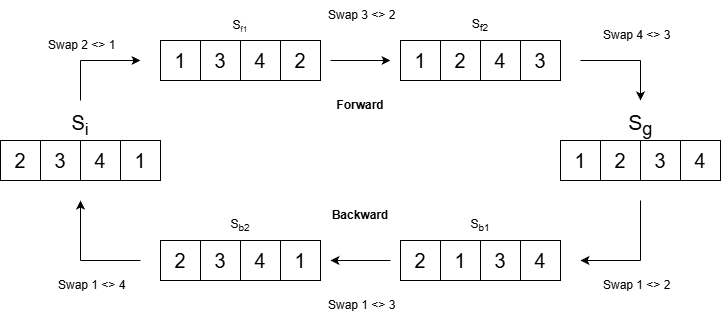
\includegraphics[scale=0.5]{path_relinking.png}
        \caption[\small{Diagrama de Path Relinking}]{\label{FigPR} \small{Representação do caminho entre $S_i$ e $S_g$.}}
    }
\end{figure}
\vspace{-0.5cm}

\paragraph{} No contexto do VRPTW, o \textit{Path Relinking} atua como um mecanismo de cooperação de alto nível ao permitir a sinergia estrutural, combinando a eficiência de sequenciamento de uma solução com a estrutura de particionamento de veículos de outra para criar rotas que nenhum agente isolado seria capaz de conceber. Além disso, a técnica possibilita a exploração de vizinhanças distantes, uma vez que, ao contrário de buscas locais tradicionais que exploram apenas o entorno imediato, o PR investiga uma região específica do espaço de busca delimitada por duas soluções de elite, focando o esforço computacional em áreas comprovadamente promissoras.

\paragraph{} Outro fator determinante é a sua capacidade de facilitar o escape de ótimos locais, pois a trajetória entre as soluções pode atravessar vales de soluções inviáveis ou de baixa qualidade para alcançar picos de aptidão mais elevados, agindo como um catalisador para a convergência global do sistema multiagente. Dessa forma, o PR não é apenas um método de busca, mas uma filosofia de cooperação que utiliza o conhecimento acumulado por diferentes agentes especialistas para sintetizar soluções superiores, mitigando as fraquezas individuais observadas em execuções isoladas. 

\paragraph{} Como seus operadores e manipuladores de soluções são relativamente simples, o PR é menos custoso computacionalmente que uma meta-heurística, seu esforço reside majoritariamente na verificação das funções de custo. Este é seu ponto forte, mas também ponto fraco, uma vez que depende de boas soluções como entrada para melhorá-las ainda mais. É evidente, portanto, que deve ser usada em combinação com outros algoritmos, idealmente ao final das etapas.

\section{Aprendizado por Reforço}
\label{sec:rl}

\paragraph{} O Aprendizado por Reforço (\textit{Reinforcement Learning} - RL) é uma área do aprendizado de máquina que se preocupa com a forma como agentes inteligentes devem tomar ações em um ambiente a fim de maximizar uma recompensa acumulada. Diferente do aprendizado supervisionado, que se baseia em um conjunto de dados rotulados, fundamenta-se na experiência direta do agente, que aprende por meio de um processo de tentativa e erro ao interagir com o ambiente \cite{Sutton18}.

\paragraph{} A estrutura básica de um problema de RL é frequentemente modelada como um Processo de Decisão de Markov, que envolve os seguintes componentes fundamentais:

\begin{itemize}
    \item \textbf{Agente (\textit{Agent}):} O tomador de decisão que observa o ambiente e executa ações.
    \item \textbf{Ambiente (\textit{Environment}):} O contexto externo com o qual o agente interage.
    \item \textbf{Estado (\textit{State}):} Uma representação da situação atual do ambiente em um determinado instante. No contexto de otimização, o estado pode refletir a qualidade da solução atual, como o número de veículos e a distância total.
    \item \textbf{Ação (\textit{Action}):} O conjunto de decisões possíveis que o agente pode tomar.
    \item \textbf{Recompensa (\textit{Reward}):} Um sinal numérico de \textit{feedback} enviado pelo ambiente após uma ação, que indica o sucesso ou fracasso daquela decisão em relação ao objetivo final.
\end{itemize}

\paragraph{} O objetivo do RL é encontrar uma política ($\pi$), que é um mapeamento de estados para ações que maximizem o retorno esperado a longo prazo. Um conceito crítico neste processo é o equilíbrio entre exploração (\textit{exploration}), onde o agente testa novas ações para descobrir sua utilidade, e explotação (\textit{exploitation}), onde o agente utiliza o conhecimento já adquirido para escolher as ações que renderam as maiores recompensas anteriormente.

\paragraph{} Um dos mais clássicos algoritmos de RL, O Q-Learning \cite{Watkins92} é do tipo \textit{off-policy} e \textit{model-free}, o que significa que ele pode aprender a política ótima de tomada de decisão sem a necessidade de um modelo prévio das transições do ambiente ou das probabilidades de recompensa. O ``Q'' na nomenclatura refere-se à Qualidade (ou valor de utilidade), representando o quão proveitosa é uma determinada ação em um estado específico.

\begin{figure}[H]
    \centering
    \begin{tikzpicture}[
        x=1cm,
        y=1cm,
        >=Stealth,
        frame/.style={dash pattern=on 2pt off 2pt, line width=0.4pt},
        box/.style={
            draw,
            rounded corners=2pt,
            line width=0.5pt,
            fill=gray!12,
            align=center,
            inner xsep=1.5pt,
            inner ysep=0.6pt,
            minimum height=0.9cm
        },
        flow/.style={-Stealth, line width=0.5pt}
    ]
        % Canvas and split between agent side (left) and environment side (right).
        \draw[frame] (-0.45,0) rectangle (5,7);

        \node[box, minimum width=3cm] (agent) at (2.5,5.5) {Agente de Atualização\\[-8pt]da Função-Q};
        \node[box, minimum width=3cm] (reward) at (2.5,3.5) {Avaliação de\\[-8pt]Recompensa/Penalidade};
        \node[box, minimum width=2cm] (actions) at (2.5,1.5) {Conjunto de\\[-8pt]Ações Possíveis};
        \node[box, minimum width=2cm] (obs) at (7.0,5.5) {Observação};
        \node[box, minimum width=2cm] (fav) at (7.0,1.5) {Ação Mais\\[-8pt]Favorável};
        \node[box, minimum width=2cm] (env) at (9.0,3.5) {Ambiente};

        \draw[flow] (obs.west) -- (agent.east);
        \draw[flow] (env.north) |- (obs.east);
        \draw[flow] (agent.south) -- (reward.north);
        \draw[flow] (reward.south) -- (actions.north);
        \draw[flow] ([xshift=0.45cm]actions.north) -- ([xshift=0.45cm]reward.south);
        \draw[flow] (actions.east) -- (fav.west);
        \draw[flow] (fav.east) -| (env.south);
        \coordinate (leftloop) at ([xshift=-0.2cm]reward.west);
        \draw[flow] (agent.west) -- (leftloop |- agent.west) -- (leftloop |- actions.west) -- (actions.west);

    \end{tikzpicture}
    \caption[\small{Visão geral do Q-Learning}]{\label{FigQL1} \small{Esquema de interação entre agente e ambiente no processo de aprendizagem.}}
\end{figure}
\vspace{-0.5cm}

\paragraph{} O núcleo do algoritmo consiste em estimar os valores da função $Q(s, a)$, que mensura a recompensa total esperada a longo prazo que um agente pode obter ao realizar a ação $a$ partindo do estado $s$. Em problemas com espaços de estados discretos, esses valores são armazenados em uma estrutura de dados conhecida como Tabela-Q (\textit{Q-Table}), onde as linhas representam os estados do sistema e as colunas as ações possíveis.

\begin{figure}[H]
    \centering
    \begin{tikzpicture}[
        >=Stealth,
        box/.style={
            draw,
            rounded corners=2pt,
            line width=0.5pt,
            fill=gray!12,
            align=center,
            inner xsep=2pt,
            inner ysep=1pt,
            minimum width=2.8cm,
            minimum height=1.0cm
        },
        flow/.style={-Stealth, line width=0.5pt}
    ]
        \node[box] (s1) at (0,0) {Inicializar\\[-8pt]Tabela-Q};
        \node[box] (s2) at (0,-1.8) {Escolher uma\\[-8pt]ação};
        \node[box] (s3) at (0,-3.6) {Executar\\[-8pt]ação};
        \node[box] (s4) at (0,-5.4) {Medir\\[-8pt]recompensa};
        \node[box] (s5) at (0,-7.2) {Atualizar\\[-8pt]Tabela-Q};

        \draw[flow] (s1.south) -- (s2.north);
        \draw[flow] (s2.south) -- (s3.north);
        \draw[flow] (s3.south) -- (s4.north);
        \draw[flow] (s4.south) -- (s5.north);
        \draw[flow] (s5.east) -- ++(1.9,0) -- ++(0,5.4) -- (s2.east);
        \node[font=\scriptsize, align=center, rotate=90] at (3.95,-4.5)
            {Após múltiplas iterações,\\[-1pt]uma boa Tabela-Q está pronta};
    \end{tikzpicture}
    \caption[\small{Algoritmo básico de Q-Learning}]{\label{FigQL2} \small{Diagrama do algoritmo de atualização do valor-$Q$.}}
\end{figure}
\vspace{-0.5cm} % Ajuste este valor conforme necessário para aproximar o texto

\paragraph{} O aprendizado ocorre através da atualização iterativa dos valores-Q (\textit{Q-values}) conforme o agente explora o ambiente. Essa atualização fundamenta-se na Equação de Bellman, que ajusta o valor atual com base na recompensa imediata recebida e na melhor estimativa de recompensas futuras:

\begin{equation}
    \label{EqQLearning}
    Q(s, a) \leftarrow Q(s, a) + \alpha [r + \gamma \max_{a'} Q(s', a') - Q(s, a)]
\end{equation}

\paragraph{} Nesta formulação, os parâmetros de controle desempenham papéis cruciais:

\begin{itemize}
    \item \textbf{Taxa de Aprendizado ($\alpha$):} Determina o quanto a nova informação substitui o conhecimento antigo.
    \item \textbf{Recompensa Imediata ($r$):} É o \textit{feedback} numérico direto recebido do ambiente após a execução de uma ação. Representa o ganho instantâneo e serve como a base factual para atualizar a estimativa de qualidade daquela ação.
    \item \textbf{Fator de Desconto ($\gamma$):} Define a importância das recompensas futuras em relação às imediatas.
    \item \textbf{Diferença Temporal:} O termo entre colchetes representa o erro de predição, ou seja, a diferença entre o valor que o agente esperava e o que ele efetivamente percebeu após a transição para o novo estado $s'$.
\end{itemize}

\paragraph{} Para que o algoritmo seja eficaz, o agente deve balancear a busca por novos conhecimentos com o uso do conhecimento já adquirido. A estratégia mais comum é a $\epsilon-greedy$, onde com uma probabilidade $\epsilon$ o agente escolhe uma ação aleatória (exploração) e com probabilidade $1 - \epsilon$ ele seleciona a ação com o maior valor-Q atual para aquele estado (explotação). Ao final do processo de treinamento, a Tabela-Q converge para uma representação da estratégia ótima, permitindo que o sistema, ao se deparar com uma determinada configuração do problema, saiba as melhores ações a serem tomadas.

\section{Avaliação estatística de desempenho algorítmico}
\label{sec:avaliacao_estatistica}

\paragraph{} A avaliação de desempenho de meta-heurísticas aplicadas a problemas de otimização combinatória, como o VRPTW, impõe desafios metodológicos devido à natureza estocástica inerente a esses algoritmos. A comparação direta de métricas de tendência central, como a média aritmética, é insuficiente para atestar a superioridade de um método sobre outro, uma vez que flutuações amostrais decorrentes de inicializações aleatórias (\textit{seeds}) podem distorcer os resultados. Torna-se imperativo, portanto, o emprego de testes de hipóteses estatísticas.

\paragraph{} Visto que as distribuições de custos de rotas e tempos de processamento computacional raramente atendem aos pressupostos clássicos de normalidade (distribuição Gaussiana) e homogeneidade de variância, a aplicação de testes paramétricos tradicionais, como o teste $t$ de Student ou a clássica ANOVA, torna-se inadequada. Em cenários de \textit{benchmarks} múltiplos avaliados sobre um mesmo conjunto de instâncias correlacionadas (amostras pareadas), a literatura prescreve a utilização de abordagens não-paramétricas baseadas na ordenação de resultados por postos (\textit{ranks}).

\subsection{Teste de Friedman}

\paragraph{} O Teste de Friedman configura-se como a alternativa não-paramétrica à ANOVA para medidas repetidas. Ele é utilizado para detectar diferenças globais significativas entre múltiplos tratamentos aplicados a diversos blocos de teste. No contexto computacional, os tratamentos correspondem aos diferentes algoritmos ou arquiteturas implementadas (tais como SA, TS, GA, MAS e MAS-RL), enquanto os blocos representam as instâncias de teste do \textit{benchmark} (como as instâncias de Solomon).

\paragraph{} O procedimento do teste consiste em ordenar os algoritmos individualmente dentro de cada instância, atribuindo o posto $1$ ao melhor desempenho (ex: menor número de veículos) e o posto $k$ ao pior (sendo $k$ o número total de algoritmos analisados). Em caso de empates numéricos, atribui-se a média dos postos em disputa a cada um dos algoritmos empatados. A hipótese nula ($H_0$) do teste estabelece que as amostras provêm da mesma população contínua, ou seja, assume que as distribuições dos postos de todos os métodos avaliados são estatisticamente equivalentes. Por sua vez, a hipótese alternativa ($H_1$) dita que existe uma diferença estatisticamente significativa na distribuição dos postos de, pelo menos, um dos algoritmos no grupo avaliado em relação aos demais.

\paragraph{} A estatística do teste ($\chi^2_F$) é computada com base na soma dos postos de cada algoritmo, avaliando a disparidade desses valores em relação ao cenário de equivalência estrita. Se o \textit{p-valor} associado gerado pela distribuição do teste for inferior ao nível de significância preestabelecido $\theta$ (tipicamente adotado como $0.05$ ou $0.10$), rejeita-se a hipótese nula.

\subsection{Teste Post-Hoc de Nemenyi}

\paragraph{} A rejeição da hipótese nula no Teste de Friedman estabelece apenas a existência de uma disparidade de desempenho no grupo geral de algoritmos (\textit{omnibus test}), falhando em especificar quais pares exatos de métodos diferem significativamente entre si. Para realizar tais comparações múltiplas par a par, mantendo o controle rigoroso sobre a inflação do Erro do Tipo I (falsos positivos), exige-se a aplicação de um teste \textit{post-hoc}. Neste escopo, o Teste de Nemenyi é a metodologia padrão recomendada para a área de aprendizado de máquina e otimização.

\paragraph{} O Teste de Nemenyi determina que o desempenho de dois algoritmos é considerado significativamente distinto se a diferença absoluta entre os seus \textit{ranks} médios superar um limiar matemático rigoroso denominado Diferença Crítica (CD, do inglês \textit{Critical Difference}). O valor numérico da CD é calculado de acordo com a equação:

$$\text{CD} = q_\alpha \sqrt{\frac{k(k + 1)}{6N}}$$

\paragraph{} Onde $q_\alpha$ representa o valor crítico tabelado baseado na distribuição de amplitude \textit{Studentized Range} para o nível de significância $\alpha$ (ou $\theta$) adotado; $k$ representa o número de algoritmos comparados no experimento; e $N$ consiste no número de instâncias ou blocos independentes avaliados.

\paragraph{} Graficamente, as conclusões deste teste \textit{post-hoc} são comumente sumarizadas e representadas pelo Diagrama de Diferença Crítica (\textit{Critical Difference Diagram}). Nele, os métodos computacionais são dispostos em um eixo horizontal de acordo com o seu respectivo \textit{rank} médio de desempenho. Algoritmos que não apresentam diferenças estatísticas significativas são agrupados por uma linha espessa de conexão, oferecendo uma percepção visual inequívoca acerca do ranqueamento global, das distâncias de performance e das reais equivalências operacionais entre os sistemas propostos.

% ---------------------------------------------------------------
% Chapter 3 - Desenvolvimento
% ---------------------------------------------------------------
\chapter{Método Proposto}
\label{cap3}
\paragraph{}Este capítulo descreve a materialização metodológica da pesquisa, mapeando as fases das implementações executadas. A primeira estruturação analítica está descrita na \autoref{sec:etapas_iniciais} com pautas iniciais como pré-processamento de datasets cartesianos, extração dos parâmetros georreferenciados para as estruturas na modelagem computacional e a verificação das rotinas em base conhecida. Em progressão, a \autoref{sec:inc_sma} introduz e apresenta esquematicamente o ambiente multiagente estabelecido através dos componentes unificados baseados no \textit{framework Mesa}, elucidando o comportamento da seleção cooperativa das soluções e o intermédio do \textit{Path Relinking}. O avanço do paradigma do sistema inteligente colaborativo culmina na \autoref{sec:hiperheuristica} com o controle das execuções repassado para as bases do Q-Learning, estruturado com recompensas dinâmicas, decaimento de aleatoriedade perante convergência nas iterações e gestão estocástica adaptativa.

\section{Etapas iniciais}
\label{sec:etapas_iniciais}

\paragraph{} As fases preliminares do desenvolvimento focaram na construção da arquitetura base do sistema. Foram implementadas as rotinas de entrada e saída de dados, responsáveis pela leitura dos \textit{datasets} e dos arquivos de solução de referência (\textit{benchmarks}), além de módulos para a visualização gráfica de rotas e monitoramento de desempenho.

\paragraph{} Um componente crítico nesta etapa foi a função custo compartilhada, desenvolvida de forma modular para garantir que a avaliação das rotas fosse consistente entre os diferentes algoritmos testados. Para validar a implementação, utilizou-se como referência a \textbf{instância RC201} de Solomon (resultado e procedimentos seguidos para alcançar tal, respectivamente em \cite{Sintef100, Mester05}). A figura abaixo apresenta a distribuição espacial dos clientes nesta instância.

\begin{figure}[H]
    \centering
    \parbox[htb]{13.0cm}
    {
        \centering
        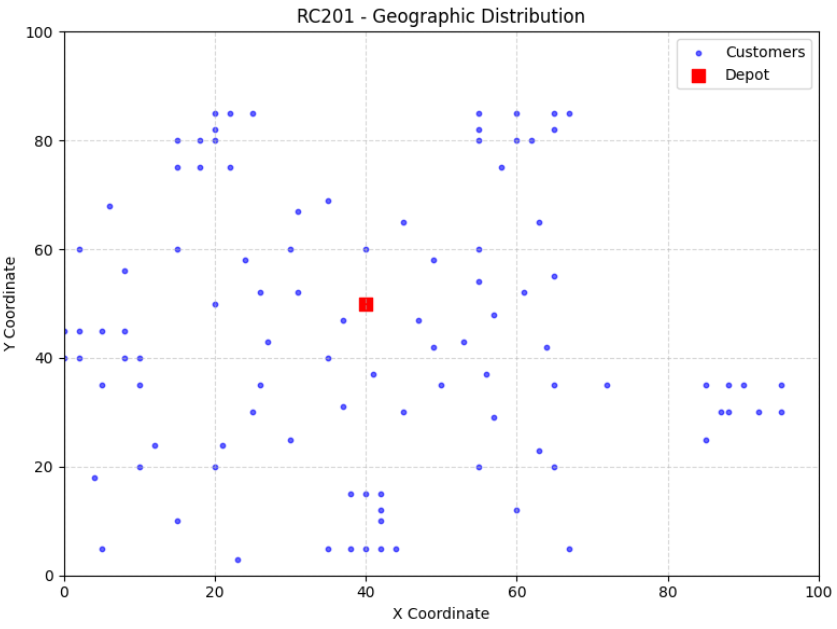
\includegraphics[scale=0.5]{solomon_rc201.png}
        \caption[\small{Distribuição da instância RC201}]{\label{FigRC201} \small{Distribuição espacial dos clientes e do depósito na instância RC201 de Solomon.}}
    }
\end{figure}
\vspace{-0.5cm}

\paragraph{} A validação da função custo ocorreu por meio da leitura da melhor solução conhecida para a RC201. Ao processar essa solução e comparar os resultados obtidos com os indicadores do \textit{benchmark}, confirmou-se a integridade do cálculo de custo. A figura abaixo ilustra o conjunto de rotas ótimas para este cenário.

\begin{figure}[H]
    \centering
    \parbox[htb]{13.0cm}
    {
        \centering
        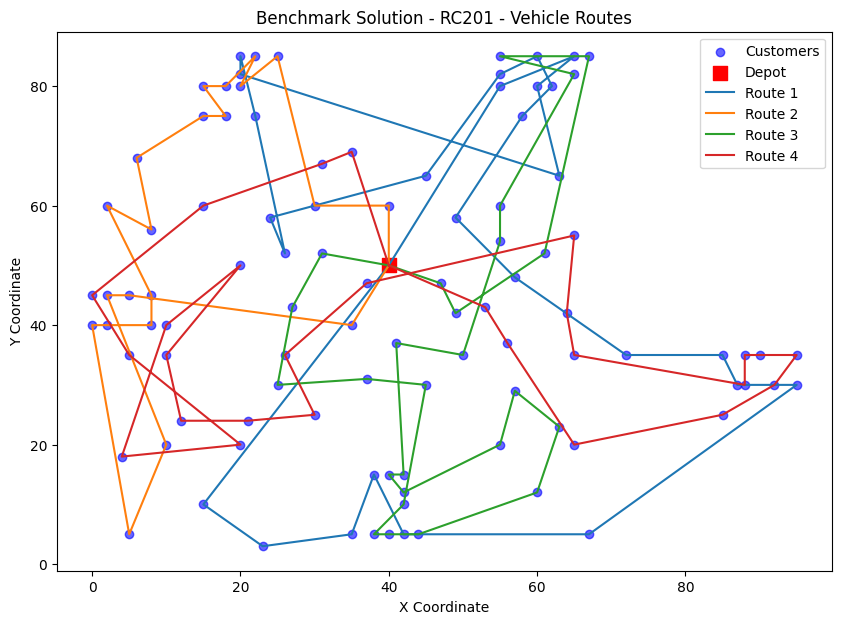
\includegraphics[scale=0.5]{solucao_otima_rc201.png}
        \caption[\small{Rotas ótimas da instância RC201}]{\label{FigRC201Opt} \small{Visualização do conjunto de subrotas da melhor solução conhecida para a instância RC201.}}
    }
\end{figure}
\vspace{-0.5cm}

\paragraph{} Por fim, foram estruturadas as classes base para os algoritmos meta-heurísticos. Essa arquitetura orientada a objetos permitiu a execução dos testes preliminares e a coleta dos primeiros dados para análise comparativa.

\paragraph{} Um ponto importante a se notar é a escolha de não separar rotas em viável ou inviável ao longo dos algoritmos. Todas as rotas foram consideradas realizáveis, de forma que a inserção de retorno ao depósito nas rotas se dá pela verificação da impossibilidade de seguir para um próximo cliente, seja pela limitação de carga ou temporal.

\section{Implementação de sistema multiagente}
\label{sec:inc_sma}

\paragraph{} A arquitetura do sistema proposto foi desenvolvida utilizando o \textit{framework Mesa}, que permite a modelagem de agentes autônomos em um ambiente controlado. No contexto deste trabalho, o MAS atua como uma camada de coordenação que integra as meta-heurísticas independentes, transformando-as em agentes especialistas que colaboram para a otimização do VRPTW.

\subsection{Arquitetura e componentes do sistema}

\paragraph{} O modelo é estruturado em três componentes principais, conforme implementado na classe \texttt{VRPOptimizationModel}:

\begin{itemize}
    \item \textbf{Agentes Especialistas (\textit{HeuristicAgent}):} Cada instância representa uma meta-heurística (SA, TS ou GA) que atua de forma independente. Em cada ciclo de execução (\textit{step}), o agente recupera uma solução promissora do \textit{pool} de elite para servir como uma solução inicial (evidentemente, em estado melhor que uma solução inicial puramente aleatória), executa sua lógica de busca e devolve o resultado aprimorado ao sistema.
    \item \textbf{Memória Compartilhada (\textit{ElitePool}):} Funciona como um quadro negro que armazena as melhores soluções encontradas por todos os agentes. O \textit{pool} possui um tamanho fixo, garantindo que apenas as soluções com menor custo (considerando o número de veículos $K$ e distância total $D$) sejam mantidas e compartilhadas. Para garantir variabilidade entre as soluções, também foi implementado mecanismo que evita a inserção de soluções demasiadamente parecidas com as já presentes na \textit{pool}
    \item \textbf{Mecanismo de Coordenação e Sincronização:} O modelo executa os agentes em paralelo, inserindo, se aptas, suas soluções no \textit{ElitePool} ao final do ciclo.
\end{itemize}

\subsection{Cooperação e a estratégia de Path Relinking}

\paragraph{} A verdadeira cooperação no SMA ocorre através do método \texttt{run\_path\_relinking}. Diferente de uma execução paralela simples, este sistema implementa uma busca cooperativa onde duas soluções de elite são combinadas:

\begin{enumerate}
    \item \textbf{Seleção por Diversidade:} O sistema seleciona a melhor solução atual (\textit{source}) e a compara com outros candidatos no \textit{ElitePool}, escolhendo aquele com maior distância de \textit{Hamming} (maior diversidade) como alvo (\textit{target}).
    \item \textbf{Exploração Bidirecional:} Adotou-se a estratégia de \textit{Path Relinking} bidirecional, na qual a exploração ocorre simultaneamente em dois sentidos: da solução \textit{source} em direção à \textit{target} e vice-versa. Essa abordagem dobra as trajetórias exploradas entre os dois pontos de elite, permitindo que o algoritmo investigue vizinhanças distintas que poderiam ser negligenciadas em uma busca unidirecional.
    \item \textbf{Permutação e Reavaliação:} Durante a trajetória, a técnica gera caminhos intermediários permutando clientes e reavaliando a função de custo a cada passo. O uso do critério bidirecional acelera o encontro de soluções que compartilham características de ambos os genitores de elite.
    \item \textbf{Sintetização de Soluções:} Se uma solução intermediária superar as originais em termos de custo (veículos $K$ ou distância $D$), ela é adicionada ao \textit{pool}, permitindo que o sistema escape de ótimos locais ao fundir características de rotas distintas geradas por agentes diferentes.
\end{enumerate}

\paragraph{} O fluxo operacional do MAS está sintetizado na \autoref{FigFluxMASSimples}.

\begin{figure}[H]
    \centering
    \begin{tikzpicture}[
        >=Stealth,
        node distance=0.75cm and 1.2cm,
        box/.style={
            draw,
            rounded corners=2pt,
            line width=0.5pt,
            fill=gray!12,
            align=center,
            inner xsep=3pt,
            inner ysep=2pt,
            minimum height=0.95cm,
            text width=4.6cm,
            font=\scriptsize
        },
        smallbox/.style={
            draw,
            rounded corners=2pt,
            line width=0.5pt,
            fill=gray!12,
            align=center,
            inner xsep=2pt,
            inner ysep=2pt,
            minimum height=0.9cm,
            text width=2.8cm,
            font=\scriptsize
        },
        flow/.style={-Stealth, line width=0.5pt}
    ]
        % Definição dos nós do fluxo principal
        \node[box] (start) {Início do \textit{step} do MAS};
        \node[box, below=of start] (seed) {Obter sementes iniciais para os agentes a partir do \textit{ElitePool}};
        \node[box, below=of seed] (dispatch) {Despachar SA, TS e GA em paralelo};

        % Nós dos agentes em paralelo
        \node[smallbox, below left=of dispatch] (sa) {\textit{Processo} 1\\Agente SA};
        \node[smallbox, below=of dispatch] (ts) {\textit{Processo} 2\\Agente TS};
        \node[smallbox, below right=of dispatch] (ga) {\textit{Processo} 3\\Agente GA};

        % Fluxo linear pós-sincronização
        \node[box, below=1.0cm of ts] (merge) {Sincronizar retornos, validar factibilidade e atualizar \textit{ElitePool}};
        \node[box, below=of merge] (runpr) {Executar \textit{Path Relinking} bidirecional e inserir melhoria no \textit{pool} (se houver)};
        \node[box, below=of runpr] (end) {Encerrar \textit{step}};

        % Desenho dos fluxos e setas
        \draw[flow] (start) -- (seed);
        \draw[flow] (seed) -- (dispatch);

        \draw[flow] (dispatch) -- (sa);
        \draw[flow] (dispatch) -- (ts);
        \draw[flow] (dispatch) -- (ga);

        \draw[flow] (sa.south) |- (merge.west);
        \draw[flow] (ts.south) -- (merge.north);
        \draw[flow] (ga.south) |- (merge.east);

        \draw[flow] (merge) -- (runpr);
        \draw[flow] (runpr) -- (end);
    \end{tikzpicture}
    \caption[\small{Fluxograma do MAS}]{\label{FigFluxMASSimples} \small{Fluxo de execução do \texttt{VRPOptimizationModel} na configuração final paralela. O \textit{step} executa SA, TS e GA em paralelo, consolida soluções no \textit{ElitePool} e aplica o \textit{Path Relinking} sequencialmente antes do encerramento.}}
\end{figure}
\vspace{-0.5cm}



\paragraph{Uso de processos x threads} 

\paragraph{} Ressalta-se a limitação fundamental no uso de \textit{threads} para a paralelização em Python, que reside na presença do \textit{Global Interpreter Lock} (\textit{GIL}). O \textit{GIL} é um mecanismo de exclusão mútua que assegura que apenas uma \textit{thread} execute \textit{bytecode} Python por vez, independentemente da quantidade de núcleos de processamento disponíveis na arquitetura de hardware utilizada. 

\paragraph{} Em tarefas \textit{CPU-bound}, nas quais o processamento é predominantemente matemático e intensivo, como é o caso das meta-heurísticas aplicadas, a utilização de \textit{threads} não resulta em paralelismo efetivo. Pelo contrário, o \textit{GIL} força a alternância de contexto (\textit{context switching}) entre as \textit{threads}, introduzindo um \textit{overhead} que pode degradar o desempenho global do sistema.

\paragraph{} Para contornar esta restrição, a arquitetura deste trabalho adota o \textit{ProcessPoolExecutor}, que fundamenta-se na utilização de processos independentes. Diferente das \textit{threads}, cada processo possui seu próprio interpretador Python, seu próprio espaço de memória isolado e, crucialmente, seu próprio \textit{GIL}. Desta forma, o Sistema Operacional é capaz de escalar cada processo para um núcleo de CPU distinto, garantindo o paralelismo real e permitindo que os agentes operem de forma simultânea e eficiente durante a busca por soluções.

\paragraph{} Isto exige uma estrutura de comunicação entre processos, sincronização dos retornos e controle mais manual da memória, mas os ganhos em tempo superam significativamente os custos.

\section{Hiper-heurística baseada em Aprendizado por Reforço}
\label{sec:hiperheuristica}

\paragraph{} A evolução do sistema multiagente convencional para o modelo proposto reside na implementação da classe \texttt{VRPOptimizationModelRL}. Neste modelo, o mecanismo de coordenação deixa de executar sempre uma busca para cada agente e passa a utilizar o algoritmo \textit{Q-Learning} para orquestrar a ativação dos agentes especialistas, configurando uma abordagem de hiper-heurística baseada em aprendizado \cite{Burke13}.

\paragraph{Modelagem do Q-Learning}

\paragraph{} O agente de RL opera sobre um ciclo de percepção e ação, onde a política de decisão é refinada com base na experiência acumulada no ambiente de busca. Os componentes do modelo são definidos como segue:

\begin{itemize}
    \item \textbf{Espaço de Estados ($S$):} O estado é definido pela tupla discreta $(K, D_{bin})$. Para evitar a explosão do espaço de estados e garantir a convergência da Tabela-Q, a distância total ($D$) é discretizada em faixas (\textit{bins}) de unidades através do parâmetro \texttt{distance\_bin\_size}.
    \item \textbf{Espaço de Ações ($A$):} Corresponde à seleção de uma das três meta-heurísticas disponíveis para execução no ciclo atual: \textit{Simulated Annealing} (SA), \textit{Tabu Search} (TS) ou \textit{Genetic Algorithm} (GA).
    \item \textbf{Função de Recompensa Hierárquica ($R$):} A recompensa é estruturada para refletir a prioridade multiobjetivo do \textit{VRPTW}:
    \begin{itemize}
        \item \textbf{Redução de Frota:} Atribui-se uma recompensa massiva caso a ação resulte na diminuição do número de veículos ($K$).
        \item \textbf{Redução de Distância:} A recompensa é equivalente à magnitude da melhoria em $D$.
        \item \textbf{Penalidade por Estagnação:} Aplica-se uma pequena penalidade se a ação não gerar melhorias, incentivando a exploração de outros agentes.
    \end{itemize}
    \item \textbf{Política de Seleção:} Utiliza-se a estratégia $\epsilon$-\textit{greedy}, equilibrando a explotação do conhecimento atual com a exploração de novas trajetórias de busca. Além disso aplica-se um decaimento progressivo de $\epsilon$ ao longo dos ciclos para favorecer a convergência.
\end{itemize}



\paragraph{} A cada \textit{step} do modelo, o sistema realiza três iterações de escolha e execução. Após a execução do agente selecionado, o valor de utilidade $Q(s, a)$ é atualizado na Tabela-Q utilizando a \autoref{EqQLearning}. Paralelamente ao RL, o método \texttt{run\_path\_relinking} continua a promover a síntese de soluções de elite, agora alimentado por um \textit{pool} cujos candidatos são gerados por agentes selecionados de forma adaptativa.


\paragraph{} No método final implementado (classe \texttt{VRPOptimizationModelRL}), cada \textit{step} ocorre em duas fases. Na fase de decisão, o agente de RL seleciona \texttt{runs\_per\_step} ações por política $\epsilon$-\textit{greedy}. Na fase de execução, as ações selecionadas são despachadas em paralelo. Após a sincronização dos processos, cada solução retornada é avaliada, inserida no \textit{ElitePool} (quando viável), e o valor de utilidade $Q(s,a)$ é atualizado conforme a \autoref{EqQLearning}. Este funcionamento é ilustrado no fluxograma da \autoref{FigFluxFinalMASRL}.

\begin{figure}[H]
    \centering
    \begin{tikzpicture}[
        >=Stealth,
        node distance=0.75cm and 1.2cm,
        box/.style={
            draw,
            rounded corners=2pt,
            line width=0.5pt,
            fill=gray!12,
            align=center,
            inner xsep=3pt,
            inner ysep=2pt,
            minimum height=0.95cm,
            text width=4.6cm,
            font=\scriptsize
        },
        smallbox/.style={
            draw,
            rounded corners=2pt,
            line width=0.5pt,
            fill=gray!12,
            align=center,
            inner xsep=2pt,
            inner ysep=2pt,
            minimum height=0.9cm,
            text width=2.8cm,
            font=\scriptsize
        },
        flow/.style={-Stealth, line width=0.5pt}
    ]
        \node[box] (start) {Início do \textit{step} do MAS-RL};
        \node[box, below=of start] (select) {Para cada execução ($r=1,\dots,\texttt{runs\_per\_step}$): observar estado $(K,D_{bin})$, selecionar ação via $\epsilon$-\textit{greedy} e registrar (agente, semente)};
        \node[box, below=of select] (dispatch) {Despachar execuções selecionadas em paralelo};

        \node[smallbox, below left=of dispatch] (sa) {Processo 1\\Agente selecionado 1};
        \node[smallbox, below=of dispatch] (ts) {Processo 2\\Agente selecionado 2};
        \node[smallbox, below right=of dispatch] (ga) {Processo 3\\Agente selecionado 3};

        \node[box, below=1.0cm of ts] (merge) {Sincronizar retornos, validar factibilidade e atualizar \textit{ElitePool}};
        \node[box, below=of merge] (qupdate) {Para cada retorno: calcular recompensa, observar novo estado e atualizar $Q(s,a)$};
        \node[box, below=of qupdate] (prcheck) {Executar \textit{Path Relinking} bidirecional e inserir melhoria no \textit{pool} (se houver)};
        \node[box, below=of prcheck] (end) {Aplicar decaimento de $\epsilon$ e encerrar \textit{step}};

        \draw[flow] (start) -- (select);
        \draw[flow] (select) -- (dispatch);

        \draw[flow] (dispatch) -- (sa);
        \draw[flow] (dispatch) -- (ts);
        \draw[flow] (dispatch) -- (ga);

        \draw[flow] (sa.south) |- (merge.west);
        \draw[flow] (ts.south) -- (merge.north);
        \draw[flow] (ga.south) |- (merge.east);

        \draw[flow] (merge) -- (qupdate);
        \draw[flow] (qupdate) -- (prcheck);
        \draw[flow] (prcheck) -- (end);
    \end{tikzpicture}
    \caption[ \small{Fluxograma do MAS-RL}]{\label{FigFluxFinalMASRL} \small{Fluxo de execução do método final implementado em \texttt{VRPOptimizationModelRL}. A seleção de ações é feita pelo agente de RL, enquanto as execuções das meta-heurísticas são despachadas em paralelo. A atualização da Tabela-Q ocorre após a sincronização dos retornos, seguida pela aplicação do \textit{Path Relinking} e o decaimento de $\epsilon$.}}
\end{figure}
\vspace{-0.5cm}

\paragraph{} Abaixo, o um recorte do registro de eventos de uma execução do MAS-RL ilustra o comportamento e evolução a cada passo.

\vspace{1cm}
\begin{lstlisting}[style=mystats, basicstyle=\scriptsize\ttfamily]
Running MAS_RL (rerun) on c101.txt
MAS run=1 RL Step 1
==> State (999, 999) -> Run 1 selected SA, Run 2 selected TS, Run 3 selected TS
    |-- Run 1 agent SA result -> vehicles: 21, distance: 2094.51
    |   Update: Reward=0.00 | Q(SA) of state(999, 999) updated to 0.00
    |-- Run 2 agent TS result -> vehicles: 27, distance: 2313.44
    |   Update: Reward=-0.05 | Q(TS) of state(999, 999) updated to -0.01
    `-- Run 3 agent TS result -> vehicles: 27, distance: 2313.44
        Update: Reward=-0.05 | Q(TS) of state(999, 999) updated to -0.02
==> PR start: source (k=21, d=2094.51) -> target (k=27, d=2313.44), diversity=100
    PR candidates -> forward (k=21, d=2094.51), reverse (k=21, d=2094.51)
    PR finished: no improvement over source

MAS run=1 RL Step 2
==> State (21, 20) -> Run 1 selected SA, Run 2 selected TS, Run 3 selected SA
    |-- Run 1 agent SA result -> vehicles: 20, distance: 1837.20
    |   Update: Reward=457.32 | Q(SA) of state(21, 20) updated to 91.46
    |-- Run 2 agent TS result -> vehicles: 25, distance: 1959.95
    |   Update: Reward=-0.05 | Q(TS) of state(21, 20) updated to -0.01
    `-- Run 3 agent SA result -> vehicles: 23, distance: 2223.47
        Update: Reward=-0.05 | Q(SA) of state(21, 20) updated to 73.16
==> PR start: source (k=20, d=1837.20) -> target (k=21, d=2094.51), diversity=100
    PR candidates -> forward (k=20, d=1837.20), reverse (k=20, d=1837.20)
    PR finished: no improvement over source

...

MAS run=1 RL Step 20
==> State (18, 14) -> Run 1 selected TS, Run 2 selected TS, Run 3 selected GA
    |-- Run 1 agent TS result -> vehicles: 18, distance: 1496.46
    |   Update: Reward=-0.05 | Q(TS) of state(18, 14) updated to -0.01
    |-- Run 2 agent TS result -> vehicles: 18, distance: 1486.70
    |   Update: Reward=9.69 | Q(TS) of state(18, 14) updated to 1.93
    `-- Run 3 agent GA result -> vehicles: 18, distance: 1570.27
        Update: Reward=-0.05 | Q(GA) of state(18, 14) updated to 0.27
==> PR start: source (k=18, d=1486.70) -> target (k=18, d=1496.39), diversity=19
    PR candidates -> forward (k=18, d=1486.70), reverse (k=18, d=1478.29)
    PR improved elite pool -> (k=18, d=1478.29)
\end{lstlisting}

\paragraph{} Este registro evidencia uma pequena desvantagem da aplicação do paralelismo em um ambiente de aprendizado por reforço. A cada \textit{step}, o agente de RL seleciona múltiplas ações que são executadas em paralelo. No entanto, a atualização da Tabela-Q só ocorre após a sincronização dos retornos, o que significa que o agente de RL não tem a oportunidade de ajustar sua política entre as execuções paralelas dentro do mesmo \textit{step}.


% ---------------------------------------------------------------
% Chapter 4 - Experimentos Computacionais
% ---------------------------------------------------------------
\chapter{Experimentos Computacionais}
\label{cap4}
\paragraph{}
Este capítulo detalha o protocolo experimental adotado para a avaliação das meta-heurísticas clássicas e dos sistemas multiagente propostos. Inicialmente, a \autoref{sec:soft_hard} especifica os recursos computacionais e os pacotes de software utilizados, garantindo a reprodutibilidade dos experimentos. Na sequência, a \autoref{sec:instancias} apresenta as instâncias do \textit{benchmark} de Solomon selecionadas, enquanto a \autoref{sec:implementacao} descreve os hiperparâmetros e os detalhes de implementação que regem cada estratégia de busca. Por fim, a \autoref{sec:resultados} discute os resultados obtidos sob duas perspectivas: uma análise global agregada, que utiliza métricas de \textit{gap} normalizado para comparar a eficácia das abordagens, e uma análise individualizada por instância, que ilustra a consistência da superioridade das estratégias multiagente em diversos cenários logísticos.

\section{Software e hardware}
\label{sec:soft_hard}

\paragraph{} Uma vez que o tempo de processamento é relevante para a análise deste trabalho, serão especificadas as configurações do ambiente nos quais os testes foram realizados, bem como o código fonte utilizado, permitindo a reprodutibilidade dos resultados.
\vspace{10pt}
\begin{lstlisting}[style=mystats, basicstyle=\scriptsize\ttfamily]
Sistema Operacional: Windows 11 Home 64 bits (10.0, build 22631)
Fabricante do Sistema: Dell Inc.
Modelo do Sistema: Inspiron 14 5435
BIOS: 1.17.0
Processador: AMD Ryzen 7 7730U com Radeon Graphics (16 CPUs) - 2.0GHz
Memoria: 16384MB RAM (16GB)
\end{lstlisting}

\paragraph{} O trabalho foi desenvolvido com \texttt{Python v3.11.9}, cujos principais módulos utilizados, bem como suas versões, estão listados abaixo:
\vspace{10pt}
\begin{lstlisting}[style=mystats, basicstyle=\scriptsize\ttfamily]
matplotlib              3.10.6
Mesa                    3.3.1
numpy                   2.3.3
pandas                  2.3.2
\end{lstlisting}

\paragraph{} O código fonte se encontra em: \href{https://github.com/hugodba/TCC}{https://github.com/hugodba/TCC}


\section{Instâncias de teste}
\label{sec:instancias}

\paragraph{}Neste trabalho, os experimentos numéricos são realizados utilizando um conjunto diversificado de instâncias, englobando diferentes disposições geográficas, características de janelas de tempo e capacidades de carga. Especificamente, o conjunto de testes é composto por 12 instâncias, escolhidas de forma a constituirem um conjunto representativo: \textit{c101}, \textit{c102}, \textit{c201}, \textit{c202}, \textit{r101}, \textit{r102}, \textit{r201}, \textit{r202}, \textit{rc102}, \textit{rc103}, \textit{rc201} e \textit{rc204}. Detalhes adicionais sobre os parâmetros operacionais de cada cenário podem ser verificados no \autoref{ApendiceA}.

\section{Detalhes de implementação e parametrização}
\label{sec:implementacao}

\paragraph{} Dado que a meta-heurísticas podem continuar executando por tempo indefinido, os seus hiperparâmetros foram escolhidos balizados pela performance e estagnação. Ou seja, ao longo de testes preliminares, buscou-se um resultado ótimo e o encerramento da execução o mais rápido possível após atingi-lo. Os hiperparâmetros globais de controle do MAS e do RL também buscaram resultados ótimos, porém sem a preocupação de limitar o tempo de execução quando estagnado.

\paragraph{} Para reprodutibilidade, com o intuito de mitigar a aleatoriedade inerente às meta-heurísticas, foi implementado o uso de \textit{seeds} fixas nos geradores de números aleatórios. Tal procedimento assegura que os experimentos sejam determinísticos, permitindo a comparação direta entre diferentes rodadas e configurações. Além disso, para obtenção de maior validade estatística, dada a exstência inerente de elementos estocásticos nos métodos propostos, cada algoritmo foi executado 10 vezes para cada instância e foram levados em consideração suas médias de resultado nas análises e comparações.

\paragraph{} Quanto à instrumentação dos testes, adotou-se, para mensuração do tempo, a função \texttt{time.process\_time()}, que contabiliza exclusivamente o tempo de CPU dedicado ao processo, ignorando períodos de ociosidade (\textit{sleep}) e operações de entrada/saída (I/O). Essa escolha garante que a métrica de desempenho reflita mais fielmente o esforço computacional do algoritmo.

\begin{table}[h]
\centering
\caption[\small{Parâmetros de implementação dos experimentos.}] {\label{tab:parametros} \small{Parâmetros de implementação e controle dos experimentos.}}
\footnotesize
\begin{tabular}{lll}
\toprule
\textbf{Categoria} & \textbf{Parâmetro} & \textbf{Valor} \\
\midrule
\multirow{3}{*}{\textbf{Controles}} & Número de rodadas & 10 \\
& Seed inicial & 1 \\
\midrule
\multirow{4}{*}{\textbf{MAS}} & Tamanho do \textit{Pool} & 3 \\
& Limiar de diversidade & 10 \\
& Passos por ciclo (N\_STEPS) & 20 \\
& Política de escolha & Aleatória \\
\midrule
\multirow{3}{*}{\textbf{Meta-heurísticas}} & SA (Temp. Inicial, $\alpha$, Min, Iters) & 1800, 0.99, 3, 275 \\
& TS (\textit{Max Iters}, \textit{Tenure}, \textit{Samples}) & 480, 20, 350 \\
& GA (Pop., Gen., $P_{cross}$, $P_{mut}$) & 70, 2300, 0.7, 0.05 \\
\midrule
\multirow{3}{*}{\textbf{Meta-heurísticas (MAS)}} & SA (Temp. Inicial, $\alpha$, Min, Iters) & 1800, 0.99, 3, 28 \\
& TS (\textit{Max Iters}, \textit{Tenure}, \textit{Samples}) & 80, 20, 180 \\
& GA (Pop., Gen., $P_{cross}$, $P_{mut}$) & 70, 210, 0.7, 0.05 \\
\midrule
\multirow{6}{*}{\textbf{Q-Learning}} & $\epsilon$ (Inicial / Mínimo) & 0.8 / 0.05 \\
& Decaimento de $\epsilon$ & 0.992 \\
& $\alpha$ (Taxa de aprendizado) & 0.2 \\
& $\gamma$ (Fator de desconto) & 0.8 \\
& Bin de distância & 100 \\
& Execuções por \textit{step} & 3 \\
\bottomrule
\end{tabular}
\end{table}

\section{Resultados dos experimentos}
\label{sec:resultados}

\paragraph{} Nesta seção, serão apresentados e analisados os resultados obtidos a partir dos experimentos conduzidos, com foco na comparação entre as meta-heurísticas puras e o sistema multiagente proposto. A análise será estruturada em torno de métricas de desempenho relevantes, como o número de veículos utilizados ($K$) e o tempo de execução, além de considerar a evolução das soluções ao longo do tempo e a estabilidade dos resultados. Como objetivo secundário, a distância total percorrida ($D$) também será avaliada, porém com menor ênfase. Os dados brutos de retorno dos experiments pode ser encontrado no \autoref{ApendiceC}.


\paragraph{Desempenho global}

\paragraph{}
Para possibilitar uma análise comparativa equitativa e agregada entre instâncias com ordens de grandeza de frotas e distâncias marcadamente distintas, aplicou-se um procedimento de normalização adimensional sobre os resultados brutos. A métrica adotada fundamenta-se no cálculo do \textit{gap} relativo percentual em relação às melhores soluções conhecidas na literatura (\textit{Best Known Solutions} — BKS), conforme estabelecido pelas Equações a seguir:

$$\text{Gap } K = \frac{K_{\text{médio}} - K_{\text{ref}}}{K_{\text{ref}}}$$

$$\text{Gap } D = \frac{D_{\text{médio}} - D_{\text{ref}}}{D_{\text{ref}}}$$

\paragraph{}
Onde $K_{\text{médio}}$ e $D_{\text{médio}}$ representam as médias obtidas pelo algoritmo ao longo das 10 rodadas experimentais, enquanto $K_{\text{ref}}$ e $D_{\text{ref}}$ correspondem aos valores de referência de Solomon. Sob essa ótica, um \textit{gap} igual a zero indica o alcance exato da melhor solução da literatura. Essa metodologia viabiliza o agrupamento macro de todas as 120 execuções do lote de testes em distribuições estatísticas unificadas.

\paragraph{}
O comportamento agregado dessa normalização para a frota final de veículos ($K$) e para a distância total percorrida ($D$), considerando todos os cenários combinados, pode ser observado nos diagramas de caixa apresentados na Figura~\ref{fig:boxplot_global_k} e na Figura~\ref{fig:boxplot_global_d}, respectivamente.

\begin{figure}[H]
    \centering
    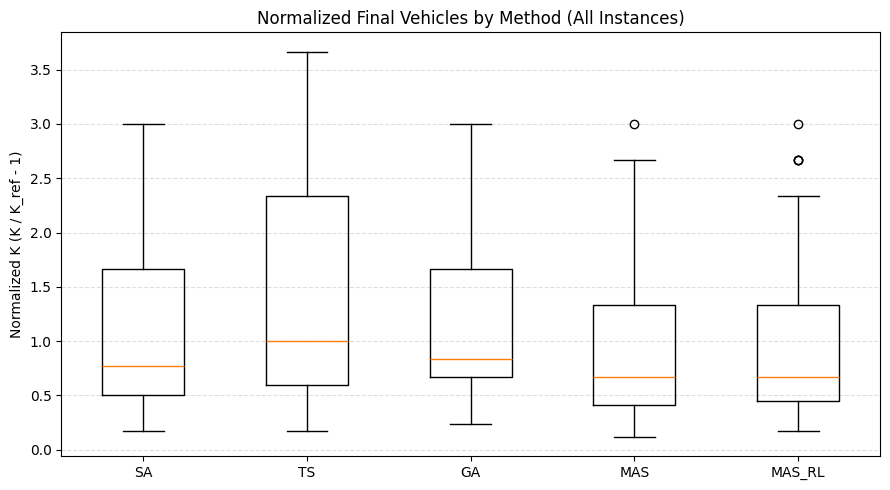
\includegraphics[width=\textwidth]{K_boxplot.png}
    \caption[\small{Distribuição do gap de frota}]{\label{fig:boxplot_global_k} \small{Distribuição do gap normalizado da frota final ($K$) por método para todas as instâncias.}}
\end{figure}

\begin{figure}[H]
    \centering
    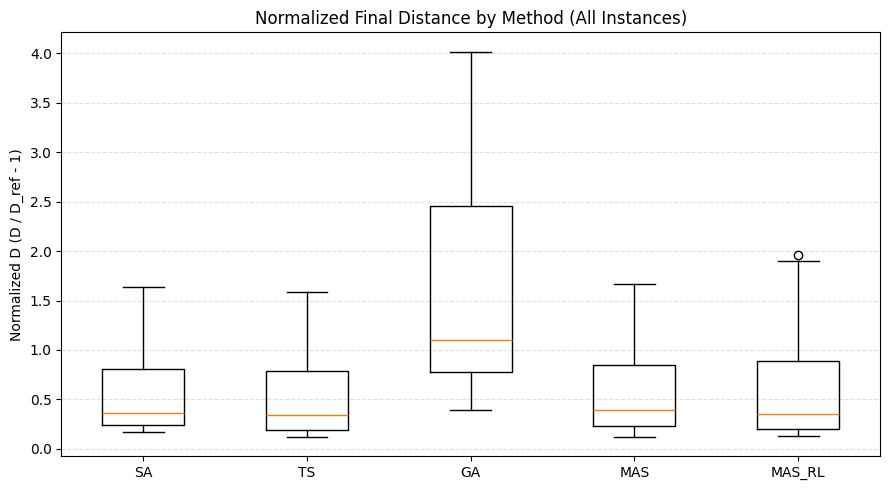
\includegraphics[width=\textwidth]{D_boxplot.png}
    \caption[\small{Distribuição do gap de distância}]{\label{fig:boxplot_global_d} \small{Distribuição do gap normalizado da distância final ($D$) por método para todas as instâncias.}}
\end{figure}

\paragraph{}
A análise macro das distribuições revela uma clara divisão de desempenho entre as abordagens tradicionais e as arquiteturas baseadas em cooperação. Ao avaliar o comportamento puramente agregado do lote completo de testes, os métodos estruturados em agência — \textit{MAS} (Sistema Multiagente) e \textit{MAS-RL} (Sistema Multiagente com Aprendizado por Reforço) — demonstram uma superioridade global evidente em relação às meta-heurísticas isoladas. Essa vantagem se traduz visualmente pelo deslocamento descendente de toda a estrutura dos diagramas de caixa, indicando uma tendência consistente de maior eficiência na minimização dos objetivos quando os solucionadores operam de forma cooperativa.

\paragraph{}
Conforme evidenciado no diagrama de frota (Figura~\ref{fig:boxplot_global_k}), a mediana do \textit{gap} de veículos para os frameworks \textit{MAS} e \textit{MAS-RL} consolida-se em patamares inferiores a 0.7, enquanto abordagens consolidadas como a Busca Tabu (\textit{TS}) e o Algoritmo Genético (\textit{GA}) operam com valores centrais próximos ou superiores a 1.0. Mais do que a redução do erro médio, as arquiteturas multiagente encolheram significativamente o intervalo interquartil da distribuição. Esse achatamento da caixa prova que o ecossistema cooperativo mitiga o risco de o algoritmo ficar aprisionado em mínimos locais medíocres ao usar as forças de cada solucionador, atingindo resultados mais consistentes, menos variáveis.

\paragraph{} No que tange à dinâmica de convergência, e não apenas ao resultado final, os métodos de agência também se destacam. A evolução temporal do \textit{gap} de frota revela que os sistemas multiagente não apenas alcançam soluções de melhor qualidade, mas o fazem de maneira mais rápida e consistente ao longo do tempo.

\paragraph{} Devido à natureza estocástica e aos tempos de execução variados entre as diferentes instâncias e rodadas, a construção dos gráficos com componente de tempo agregou os dados por meio de uma reamostragem temporal. Primeiramente, as trajetórias de cada método foram alinhadas em um \textit{grid} uniforme de 200 pontos temporais entre o instante inicial e o tempo máximo de execução, utilizando interpolação de degrau para preservar a natureza discreta das atualizações de frota.

\begin{figure}[H]
    \centering
    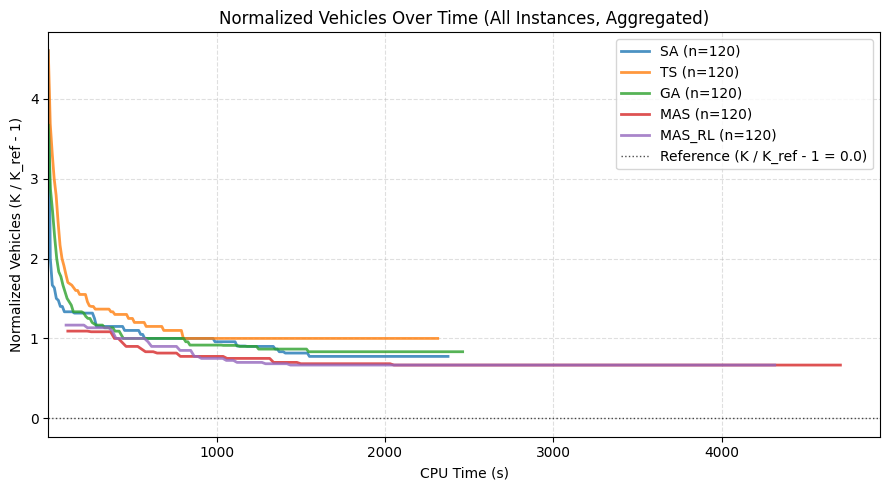
\includegraphics[width=\textwidth]{agregado_K.png}
    \caption[\small{Evolução temporal do gap de frota}]{\label{fig:convergencia_global_k} \small{Evolução temporal do gap de frota ($K$) para todas as instâncias combinadas.}}
\end{figure}

\paragraph{} É relevante observar que, desde o instante em que iniciam sua trajetória no gráfico, as abordagens multiagente posicionam-se em patamares de \textit{gap} significativamente inferiores aos métodos tradicionais. Esse comportamento decorre da natureza cooperativa do sistema: enquanto as meta-heurísticas puras são projetadas para uma convergência gradual ao longo de uma execução longa, os agentes do \textit{MAS} buscam resultados ótimos em cada um de seus steps, que são mais curtos. Além disso, eles partem de soluções iniciais enriquecidas promovidas pelo \textit{Path Relinking}. Desta forma, a arquitetura proposta mitiga a tradicional compensação (\textit{trade-off}) onde uma convergência rápida seria acompanhada por um desempenho final inferior, demonstrando que a integração entre agentes e memória compartilhada permite atingir resultados de alta qualidade de forma célere e sustentada.

\begin{figure}[H]
    \centering
    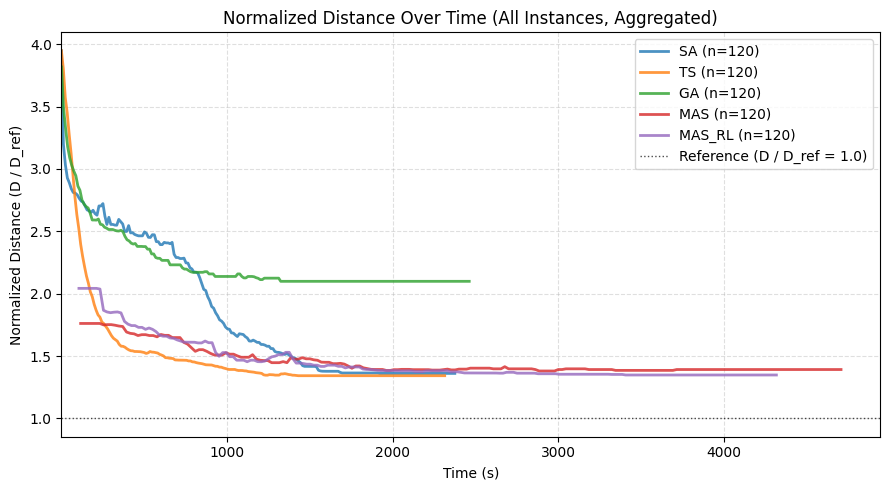
\includegraphics[width=\textwidth]{agregado_D.png}
    \caption[\small{Evolução temporal do gap de distância}]{\label{fig:convergencia_global_d} \small{Evolução temporal do gap de distância ($D$) para todas as instâncias combinadas.}}
\end{figure}

\paragraph{} Note que as linhas referentes a \textit{MAS} e \textit{MAS-RL} começam em um tempo maior, devido à arquitetura de implementação que recolhe as soluções parciais apenas após o término de cada \textit{step}, diferente das meta-heurísticas puras que atualizam a solução a cada iteração.


\paragraph{}
É imperativo destacar, contudo, a existência de um cenário de equivalência estatística primária ao comparar os resultados de qualidade de solução entre o \textit{MAS} puro e o \textit{MAS-RL}. Ambas as distribuições exibem caixas quase sobrepostas nos gráficos \ref{fig:boxplot_global_k} e \ref{fig:boxplot_global_d}, limites de dispersão equivalentes e medianas virtualmente idênticas no que tange ao \textit{gap} de frota e distância. A discussão da causa deste comportamento será detalhada adiante nas subseções subsequentes.

\paragraph{Desempenho por instâncias}

\paragraph{}
A análise detalhada por instância, consolidada na \autoref{fig:resultado_instancias}, reforça a superioridade das abordagens baseadas em sistemas multiagente em relação às meta-heurísticas isoladas. Observa-se que, independentemente da topologia da instância (tipo $C$, $R$ ou $RC$) ou do nível de restrição (Séries 1 e 2), as estratégias propostas demonstram um desempenho superior ou, no mínimo, equivalente às linhas de base tradicionais (\textit{SA}, \textit{GA}, \textit{TS}).

\begin{figure}[H]
    \centering
    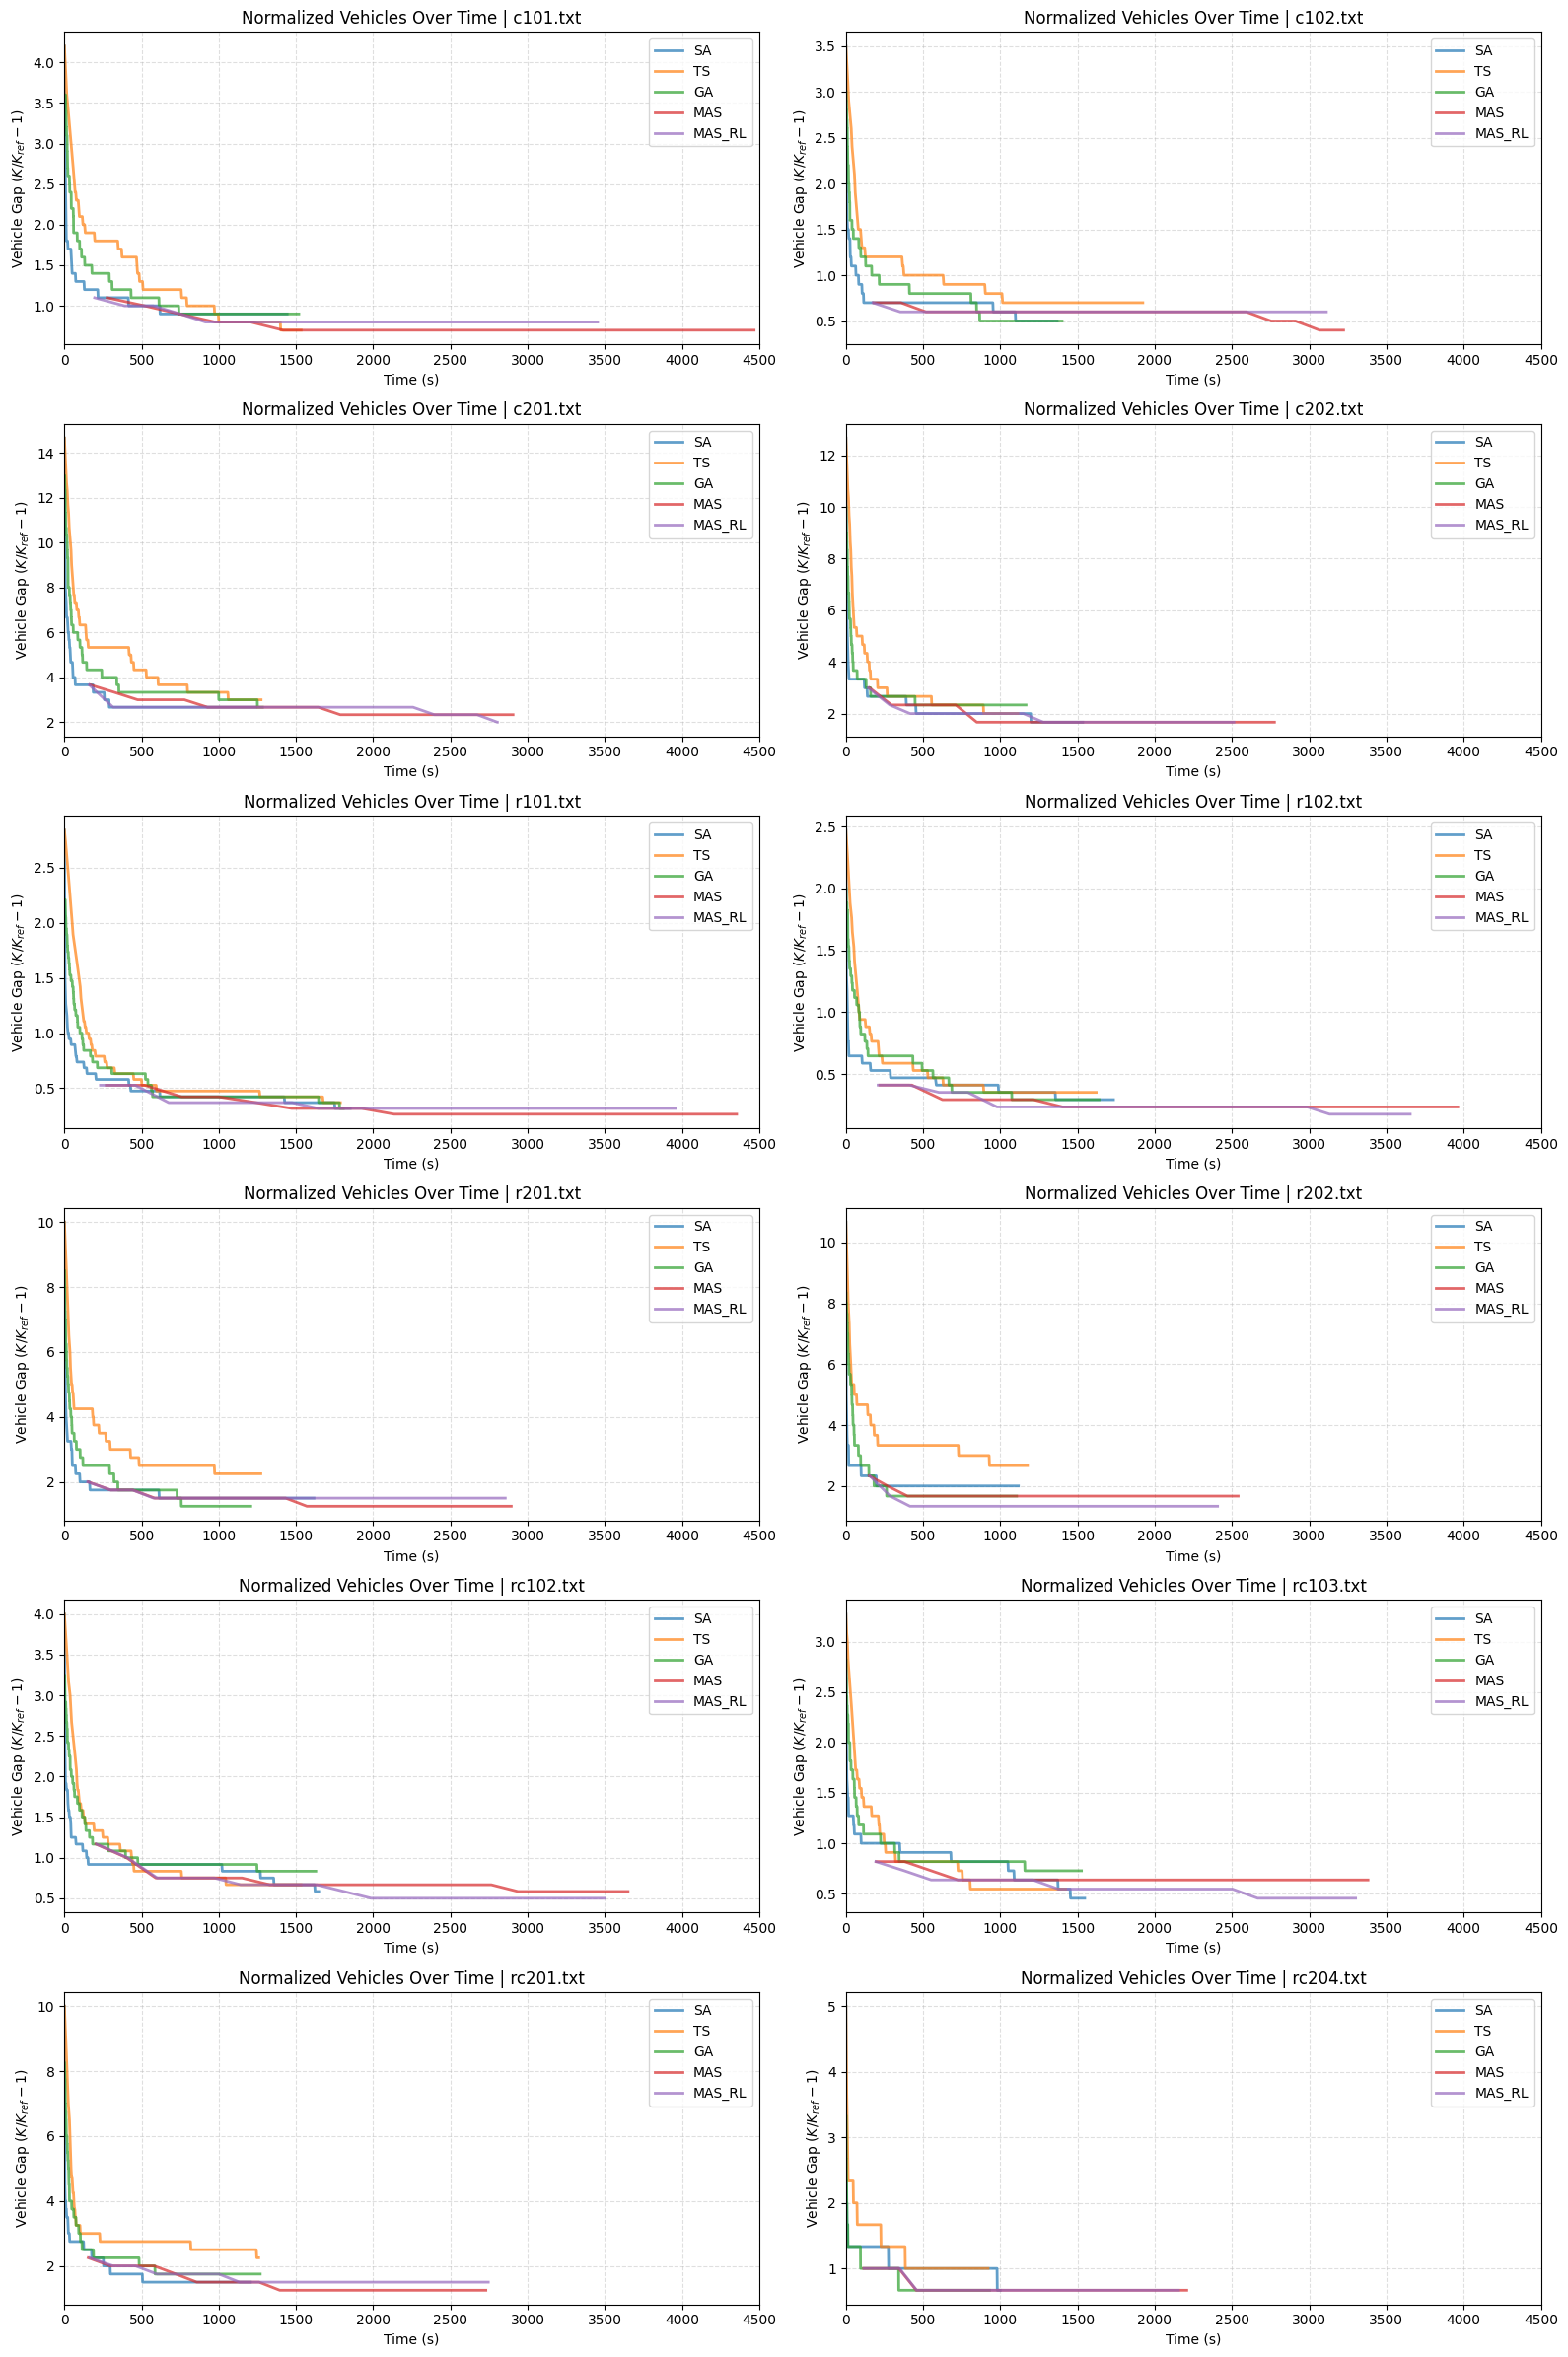
\includegraphics[width=0.9\textwidth]{resultado_instancias.png}
    \caption[\small{Análise de convergência por instância}]{\label{fig:resultado_instancias} \small{Análise de convergência por instância. As curvas ilustram o comportamento dos métodos em diferentes topologias, evidenciando a superioridade do \textit{MAS} e \textit{MAS-RL} na exploração do espaço de busca.}}
\end{figure}


\section{Análise estatística}

\paragraph{} Um teste de hipóteses foi conduzido com o objetivo de determinar se as diferenças de desempenho observadas entre os métodos propostos possuem significância estatística. Uma vez que os dados de desempenho computacional raramente seguem uma distribuição normal em otimização estocástica, e considerando que as medições foram realizadas de forma pareada nas mesmas instâncias de Solomon, abordagens não-paramétricas foram aplicadas.

\paragraph{} Neste estudo, utilizou-se um nível de significância de $\theta = 0.05$. O procedimento estatístico foi dividido em duas etapas. Inicialmente, aplicou-se o Teste de Friedman para avaliar a existência de diferenças globais no desempenho dos cinco algoritmos testados. As hipóteses formuladas para o Teste de Friedman foram:

\begin{itemize}
    \item Hipótese Nula ($H_0$): Não existe diferença significativa entre as médias dos resultados obtidos pelos métodos avaliados; todos possuem desempenhos estatisticamente equivalentes.
    \item Hipótese Alternativa ($H_1$): Existe diferença significativa entre pelo menos dois dos algoritmos testados.
\end{itemize}

\paragraph{} O Teste de Friedman reportou uma estatística $\chi^2 = 41.48$ e um p-valor associado de $2.13 \times 10^{-8}$. Como o p-valor $\ll \theta$, a hipótese nula $H_0$ é fortemente rejeitada, confirmando que há discrepância significativa na eficácia dos algoritmos perante as instâncias analisadas. Os resultados agregados que basearam este teste estão sumarizados na Tabela \ref{tab:resultados_agregados}.

\begin{table}[htbp]
    \centering
    \caption[\small{Matriz de Resultados Agregados}]{\label{tab:resultados_agregados} \small{Matriz de Resultados Agregados (Média de Veículos por Instância)}}
    \begin{tabularx}{\textwidth}{l *{5}{>{\centering\arraybackslash}X}}
        \toprule
        \textbf{Instância} & \textbf{SA} & \textbf{TS} & \textbf{GA} & \textbf{MAS} & \textbf{MAS-RL} \\
        \midrule
        \texttt{c101}  & 18.2 & 18.8 & 19.1 & 17.0 & 17.1 \\
        \texttt{c102}  & 15.2 & 17.0 & 16.5 & 15.0 & 14.8 \\
        \texttt{c201}  & 11.1 & 12.1 & 11.3 & 10.1 & 10.2 \\
        \texttt{c202}  & 8.5  & 10.6 & 9.2  & 7.6  & 7.7  \\
        \texttt{r101}  & 25.2 & 25.5 & 26.7 & 24.0 & 24.0 \\
        \texttt{r102}  & 21.1 & 21.6 & 22.5 & 20.1 & 20.5 \\
        \texttt{r201}  & 9.3  & 12.5 & 9.8  & 9.1  & 9.0  \\
        \texttt{r202}  & 7.8  & 11.1 & 7.8  & 7.2  & 7.4  \\
        \texttt{rc102} & 19.0 & 20.4 & 21.4 & 18.1 & 18.0 \\
        \texttt{rc103} & 16.3 & 17.7 & 18.7 & 16.3 & 16.2 \\
        \texttt{rc201} & 10.5 & 13.2 & 10.5 & 9.5  & 9.4  \\
        \texttt{rc204} & 5.2  & 5.8  & 5.0  & 4.6  & 4.6  \\
        \bottomrule
    \end{tabularx}
\end{table}

\paragraph{} Comprovada a diferença global, procedeu-se à segunda etapa da análise através do Teste de Nemenyi, um teste \textit{post-hoc} utilizado para identificar empiricamente, par a par, quais algoritmos apresentam diferenças significativas entre si. A Tabela \ref{tab:nemenyi_pvalues} sumariza os \textit{ranks} médios atribuídos a cada algoritmo, onde menores valores indicam maior aderência aos melhores resultados de otimização, bem como a matriz de p-valores das comparações pareadas.

\begin{table}[htbp]
    \centering
    \caption[\small{Matriz de p-valores do Teste Post-Hoc de Nemenyi e ranks médios}]{\label{tab:nemenyi_pvalues} \small{Matriz de p-valores do Teste Post-Hoc de Nemenyi e ranks médios}}
    \begin{tabular}{lcccccc}
        \toprule
        \multirow{2}{*}{\textbf{Método}} & \multirow{2}{*}{\textbf{Rank Médio}} & \multicolumn{5}{c}{\textbf{p-valor vs. Algoritmo}} \\
        \cmidrule(lr){3-7}
        & & \textbf{MAS-RL} & \textbf{MAS} & \textbf{SA} & \textbf{GA} & \textbf{TS} \\
        \midrule
        \textbf{MAS-RL} & \textbf{1.50} & -      & 1.0000 & 0.0867 & 0.0002 & 0.0000 \\
        \textbf{MAS}     & \textbf{1.54} & 1.0000 & -      & 0.1016 & 0.0003 & 0.0000 \\
        \textbf{SA}      & 3.12 & 0.0867 & 0.1016 & -      & 0.4076 & 0.1583 \\
        \textbf{GA}      & 4.25 & 0.0002 & 0.0003 & 0.4076 & -      & 0.9858 \\
        \textbf{TS}      & 4.58 & 0.0000 & 0.0000 & 0.1583 & 0.9858 & -      \\
        \bottomrule
    \end{tabular}
\end{table}

\paragraph{} Os testes indicam uma vantagem estatística notória dos sistemas multiagentes. O modelo \textit{MAS-RL} atingiu o menor \textit{rank} médio ($1.50$), intimamente seguido pelo modelo cooperativo puro MAS ($1.54$). Em contraste, as meta-heurísticas isoladas obtiveram ranks substancialmente maiores (SA: $3.12$; GA: $4.25$; TS: $4.58$).

\paragraph{} A matriz de p-valores gerada pelo Teste de Nemenyi (Tabela \ref{tab:nemenyi_pvalues}) comprova que o \textit{MAS-RL} supera significativamente tanto o TS (p-valor = $0.0000$) quanto o GA (p-valor = $0.0002$). Destaca-se também que, para a métrica de veículos, a diferença entre o \textit{MAS-RL} e o SA (p-valor = $0.0867$) encontra-se no limite tendencial, não rejeitando $H_0$ estritamente sob $\theta = 0.05$. Por fim, os resultados do \textit{MAS} e do \textit{MAS-RL} (p-valor = $1.0000$) são considerados estatisticamente equivalentes, ressaltando o ganho de robustez proveniente da arquitetura do Sistema Multiagente em si.

\paragraph{} Para ilustrar estas conclusões de forma visual, a Figura \ref{fig:cd_diagram} apresenta o Diagrama de Diferença Crítica (\textit{Critical Difference Diagram}). Os algoritmos não conectados por barras horizontais possuem diferenças estatísticas significativas de desempenho, atestando a superioridade dos arranjos cooperativos.

\begin{figure}[htbp]
    \centering
    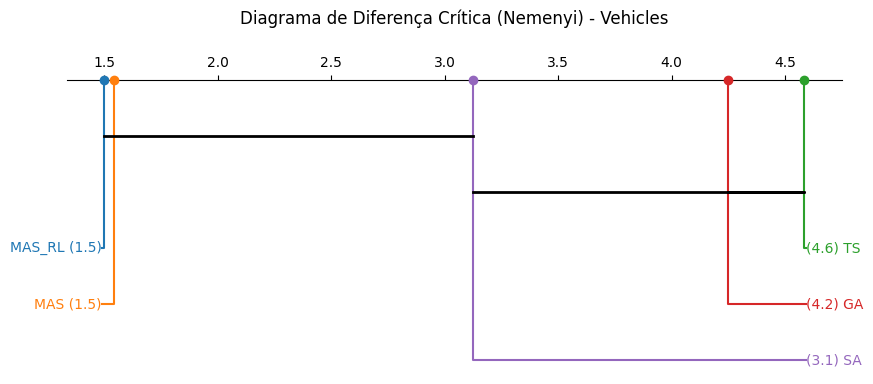
\includegraphics[width=0.85\textwidth]{cd_diagram.png}
    \caption[\small{Diagrama de Diferença Crítica (Nemenyi) para a minimização de Veículos.}]{\label{fig:cd_diagram} \small{Diagrama de Diferença Crítica (Nemenyi) para a minimização de Veículos.}}
\end{figure}

\paragraph{} Esses resultados acarretam importantes implicações práticas para o modelo desenvolvido. A superioridade estatisticamente provada do \textit{MAS} e do \textit{MAS-RL} confirma que a arquitetura cooperativa mitiga o risco de paralisação em ótimos locais, gerando configurações de frota consideravelmente melhores nas instâncias de Solomon sem que esse ganho seja decorrente do acaso. Em relação ao \textit{SA}, embora a diferença de desempenho seja evidente, a ausência de significância estatística estrita sugere que, para algumas instâncias, o SA pode alcançar resultados próximos aos sistemas multiagente, reforçando a necessidade de análises mais granulares por cenário.

% ---------------------------------------------------------------
% Chapter 5 - Conclusões
% ---------------------------------------------------------------

\chapter{Conclusão}
\label{cap5}
\paragraph{}
Este capítulo sintetiza as contribuições do presente trabalho, retomando os objetivos iniciais e apresentando as principais conclusões derivadas dos experimentos computacionais. Discute-se, ainda, as limitações observadas durante o desenvolvimento e as direções futuras para o aprimoramento do sistema multiagente proposto.

\section{Resumo dos resultados finais}

\paragraph{} A investigação realizada demonstrou que a arquitetura multiagente e sua variante com aprendizado por reforço apresentam desempenho consistentemente superior às meta-heurísticas clássicas aplicadas isoladamente. Ao permitir a exploração cooperativa do espaço de busca, o sistema proposto foi capaz de superar ou igualar o desempenho das linhas de base em todos os cenários de teste, confirmando a hipótese de que a inteligência coletiva atenua a sensibilidade das meta-heurísticas a configurações iniciais e topologias instáveis. No entanto, todos os métodos permanecem distantes das melhores soluções conhecidas.

\paragraph{} Os resultados agregados, corroborados pelas análises individuais por instância e, principalmente, o teste de hipóteses, evidenciam que a cooperação entre agentes especialistas permite uma otimização mais rápida e estável. Em relação aos métodos tradicionais, como \textit{SA}, \textit{GA} e \textit{TS}, a estrutura de agência proposta convergiu de maneira \textbf{mais consistente, mais rápida e mais eficaz}, validando a eficácia da abordagem híbrida no tratamento do \textit{VRPTW}.

\paragraph{} Reitera-se que, embora o sistema multiagente tenha demonstrado superioridade frente às abordagens isoladas, a implementação atual do \textit{Q-Learning} não apresentou ganhos significativos em relação à versão do MAS puro. Para além do dilema computacional clássico entre o número de \textit{steps} de aprendizado e o tempo disponível para as buscas locais dos agentes, essa equivalência decorre de limitações estruturais intrínsecas à modelagem concorrente.

\paragraph{} Primeiramente, o despacho paralelo de ações executadas pelos especialistas dentro de um mesmo ciclo de simulação faz com que a tabela de valores-\textit{Q} seja atualizada de forma diferida, ocorrendo apenas após a sincronização final do \textit{step}. Esse mecanismo quebra a semântica estritamente sequencial de transição de estados exigida pela \autoref{EqQLearning}, gerando um desalinhamento temporal entre a percepção do agente e o impacto real da ação no ambiente cooperativo.

\paragraph{} Ademais, a representação simplificada do espaço de estados por meio do par $(K, D_{\text{bin}})$ não se consolida como uma estatística suficiente do processo de otimização estocástica. Como a probabilidade de transição para uma nova solução depende diretamente da dinâmica interna e dos parâmetros probabilísticos de cada meta-heurística subjacente (como a temperatura do \textit{SA} ou a lista tabu), a hipótese de Markov mostra-se consideravelmente frágil. Sob essa perspectiva, o ambiente assume propriedades de um Processo de Decisão de Markov Parcialmente Observável (\textit{POMDP}), limitando a capacidade de convergência do algoritmo clássico sob recursos computacionais finitos.

\section{Oportunidades de melhoria}

\paragraph{} No âmbito do aprimoramento do trabalho em si, identificou-se a necessidade de evoluir a modelagem do estado no \textit{Q-Learning}. Uma proposta promissora, além de evidentemente aumentar o número de \textit{steps} e rever os parâmetros de aprendizado, é a implementação de herança de estados, permitindo que parte do valor-\textit{Q} de um estado anterior seja transmitido para o sucessor, acelerando a convergência do sistema. É possível, também, iniciar uma execução de otimização com uma tabela-\textit{Q} já existente (\textit{warm start}) de um treinamento anterior, o que aceleraria a convergência e os resultados. Adicionalmente, a otimização dos parâmetros das meta-heurísticas pode ser realizada através de abordagens teóricas ou empíricas mais refinadas.

\paragraph{} No que tange à análise macro do desempenho, o expressivo \textit{gap} absoluto de frota, discutido e quantificado na \autoref{sec:resultados}, consolida empiricamente as limitações associadas à heurística de fatiamento local. Conforme evidenciado nos resultados, a divisão gulosa sobre a representação em \textit{giant tour} atua importante fator de superestimação do número de veículos ($K$). Dessa forma, aponta-se como um trabalho futuro fundamental a substituição do fatiamento atual pela técnica de \textit{split} ótimo desenvolvida por \cite{prins2004simple}.

\paragraph{} No que tange à expansão do modelo e adições estruturais, sugere-se a hibridização profunda através de Algoritmos Meméticos, utilizando o conhecimento adquirido sobre o desempenho individual das meta-heurísticas para compensar fraquezas específicas de cada uma, como já realizado em parte pelo \textit{MAS}. Para aumentar a validade estatística do modelo, é importante testar o sistema em mais instâncias de dados com diferentes distribuições geográficas e números de pontos, evitando o viés de sobreajuste e aumentando o número de execuções por instância. Por fim, a aplicação em casos reais \cite{NVlabsOlist}, incorporando mapas georreferenciados e tempos de deslocamento não lineares, permitiria avaliar a robustez do \textit{MAS-RL} frente às imprevisibilidades do transporte urbano, aproximando a pesquisa acadêmica das demandas práticas do setor de logística.

\paragraph{} Outro ponto para o aumento da verossimilhança é o ajuste da função de custo para considerar explicitamente o tempo de espera, já que este fator representou uma parcela significativa do tempo total da rota nos experimentos realizados, impactando diretamente na eficiência logística.

\begin{figure}[H]
    \centering
    \parbox[htb]{13.0cm}
    {
        \centering
        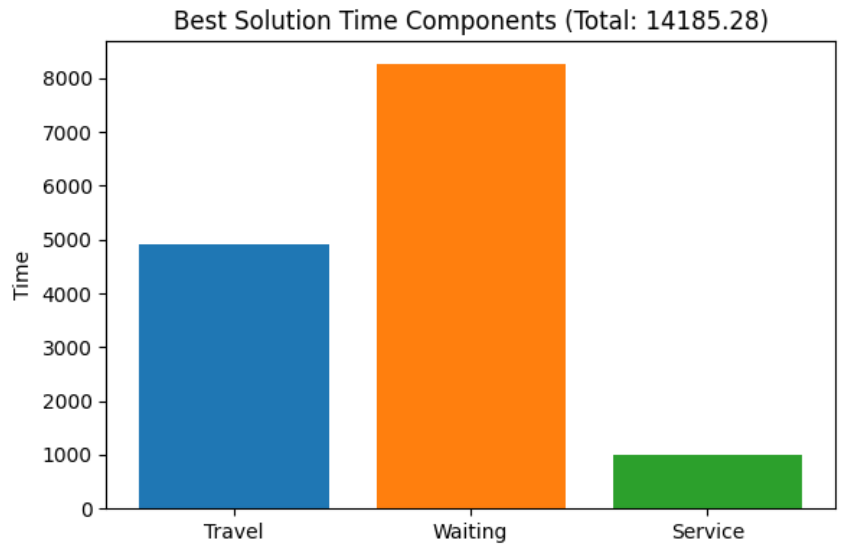
\includegraphics[scale=0.5]{waiting_time.png}
        \caption[\small{Tempo de viagem, espera e serviço}]{\label{waiting_time} \small{Tempos gastos com viagem, espera e serviço em uma execução simples de otimização para a instância \textit{R201}.}}
    }
\end{figure}
\vspace{-0.5cm} 

\paragraph{} Nota-se, conforme ilustrado na \autoref{waiting_time}, uma desproporção crítica entre o tempo de deslocamento e a ociosidade por espera, evidenciando ineficiências que impactam a viabilidade real das rotas. Visto que o tempo de serviço total é fixo, a elevada espera indica chegadas prematuras às janelas de tempo. Esse cenário reforça o desafio de sincronização temporal do \textit{VRPTW}, validando a necessidade de mecanismos de controle para mitigar a inatividade operacional.



% ---------------------------------------------------------------
% Bibliografia
% ---------------------------------------------------------------
\normalsize
\cleardoublepage
\addcontentsline{toc}{chapter}{Bibliografia}
\bibliographystyle{bibliography/coppe}
\bibliography{bibliography/biblio}

% ---------------------------------------------------------------
% Apêndices 
% ---------------------------------------------------------------
   \appendix
   % ---------------------------------------------------------------
   % Apêndice A
   % ---------------------------------------------------------------
   \chapter{Benchmark de Solomon}
   \label{ApendiceA}
    \paragraph{} No contexto de otimização e logística, as instâncias de \textit{Solomon} constituem um conjunto de problemas de teste (\textit{benchmarks}) propostos por Marius Solomon em 1987 para o VRPTW. Essas instâncias são fundamentais para aferir a eficiência de algoritmos, pois representam diferentes desafios geográficos e temporais. As nomenclaturas \textbf{C}, \textbf{R} e \textbf{RC} referem-se à disposição espacial dos clientes:

\begin{itemize}
    \item \textbf{Tipo C (\textit{Clustered}):} Os clientes estão organizados em agrupamentos (\textit{clusters}). O algoritmo deve ser eficiente em atender aos clientes de um grupo denso antes de se deslocar para o próximo. Geralmente, este perfil é considerado o de mais fácil resolução para a obtenção de rotas ótimas.
    \begin{figure}[H]
        \centering
        \parbox[htb]{13.0cm}
        {
            \centering
            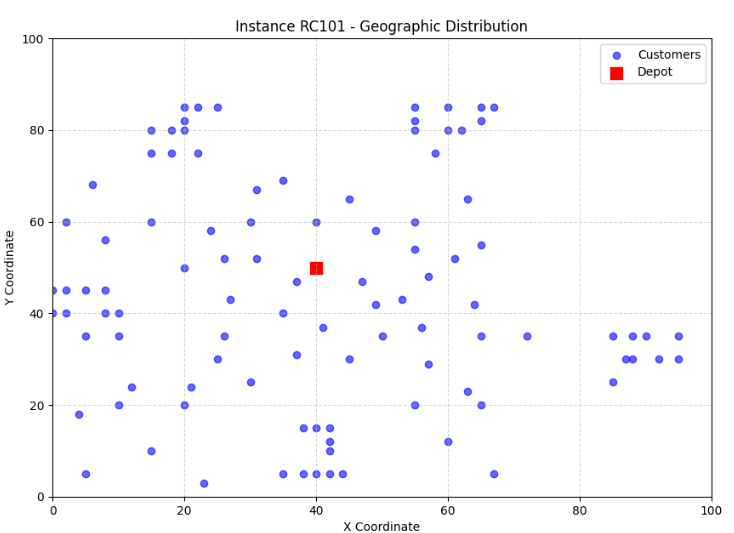
\includegraphics[scale=0.5]{C101_map.png}
            \caption[\small{Mapa da instância C101}]{\label{C101_map} \small{Distribuição geográfica dos clientes na instância \textit{Clustered} C101}}
        }
    \end{figure}
    \vspace{-0.5cm}
    
    \item \textbf{Tipo R (\textit{Random}):} Os clientes estão distribuídos de forma aleatória e uniforme no plano de coordenadas. A ausência de padrões óbvios exige que o algoritmo avalie criteriosamente as distâncias e as janelas de tempo para cada tomada de decisão.
    \begin{figure}[H]
        \centering
        \parbox[htb]{13.0cm}
        {
            \centering
            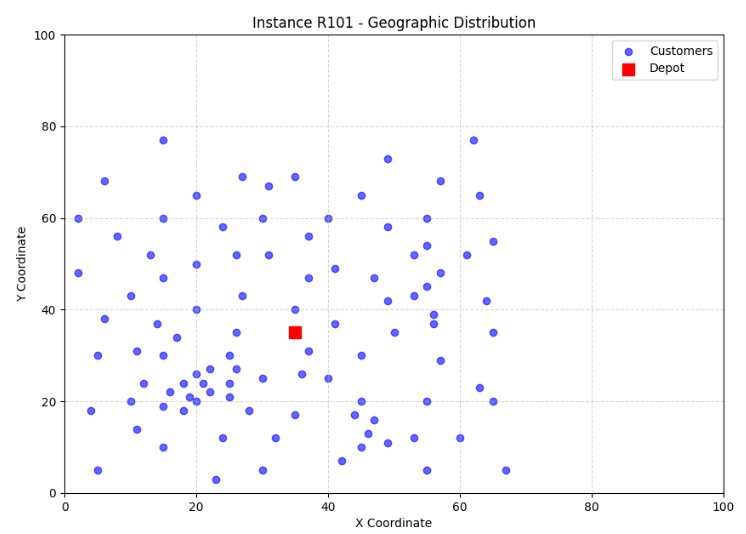
\includegraphics[scale=0.5]{R101_map.png}
            \caption[\small{Mapa da instância R101}]{\label{R101_map} \small{Distribuição geográfica dos clientes na instância \textit{Random} R101}}
        }
    \end{figure}
    \vspace{-0.5cm}
    
    \item \textbf{Tipo RC (\textit{Random-Clustered}):} Trata-se de um modelo híbrido que combina regiões de distribuição aleatória com agrupamentos definidos. Este cenário aproxima-se da realidade urbana complexa, onde centros comerciais densos convivem com áreas de entregas residenciais esparsas.
    \begin{figure}[H]
        \centering
        \parbox[htb]{13.0cm}
        {
            \centering
            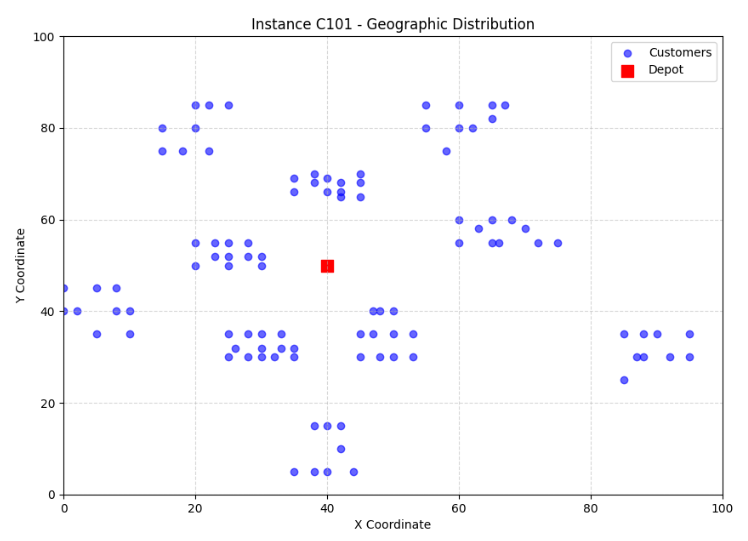
\includegraphics[scale=0.5]{RC101_map.png}
            \caption[\small{Mapa da instância RC101}]{\label{RC101_map} \small{Distribuição geográfica dos clientes na instância \textit{Random-Clustered} RC101}}
        }
    \end{figure}
    \vspace{-0.5cm}
\end{itemize}



\paragraph{} Adicionalmente, as séries \textbf{1} e \textbf{2} definem o rigor das restrições operacionais, como a capacidade de carga dos veículos e a amplitude das janelas de tempo:

\begin{itemize}
    \item \textbf{Série 1:} Apresenta restrições severas, com veículos de baixa capacidade de carga e janelas de tempo estreitas. Tais limitações resultam em rotas curtas e exigem uma frota maior para cobrir todos os pontos. Como exemplo, a instância \textit{RC101} possui uma janela de tempo média de apenas $32,08$.
    \item \textbf{Série 2:} Oferece um cenário mais flexível, com veículos de grande capacidade e janelas de tempo expandidas. Um único veículo consegue atender a uma quantidade maior de clientes, transferindo o desafio principal para a minimização da distância total percorrida. A instância \textit{RC201}, utilizada nos testes deste trabalho, possui uma janela média significativamente superior, de $128,32$.
\end{itemize}
   % ---------------------------------------------------------------
   % Apêndice B
   % ---------------------------------------------------------------
   \chapter{Estimativa para Busca Exaustiva}
   \label{ApendiceB}
    \paragraph{} Este apêndice dedica-se a estimar o tempo necessário para a obtenção de uma solução ótima, por força bruta, referente à instância RC201, a qual contém 100 clientes (incluindo o depósito). O objetivo fundamental desta seção é evidenciar a natureza combinatória da complexidade temporal intrínseca a problemas de otimização de rotas \textit{NP-hard} \cite{Garey79}, como o \textit{VRP}. Mesmo adotando a simplificação extrema do cenário para uma formulação análoga ao clássico Problema do Caixeiro Viajante (\textit{TSP}), onde um único veículo visita sequencialmente todos os destinos, as permutações resultantes exigem um esforço computacional assintoticamente proibitivo.

\paragraph{} O número de sequências possíveis para um veículo visitar todos os pontos e retornar à origem é dado por:
\[
    99! \approx 9,3326 \times 10^{155}
\]

\paragraph{} Para este cenário, assumimos um supercomputador teórico capaz de avaliar 1 bilhão ($10^9$) de soluções por milissegundo. Calculando a vazão anual desta máquina:
\[
    10^{12} \times 60 \times 60 \times 24 \times 365,25 \approx 3,15 \times 10^{19} \text{ sol./ano}
\]

\paragraph{} O tempo estimado para encontrar o ótimo absoluto seria:
\[
    \text{Tempo} = \frac{9,33 \times 10^{155}}{3,15 \times 10^{19}} \approx 2,96 \times 10^{136} \text{ anos}
\]

\paragraph{} Para compreender a magnitude deste resultado, a idade estimada do universo é de aproximadamente $13,8 \times 10^9$ anos. Outra comparação é que há ``apenas'' $10^{80}$ átomos no universo observável. Se tivéssemos começado o processamento no momento do \textit{Big Bang}, até o presente momento teríamos percorrido uma fração tão pequena do espaço de busca que ela seria estatisticamente equivalente a $0\%$.
   % ---------------------------------------------------------------

\backmatter

\end{document}
